General structure and tasks of an early warning system were already described in chapter \ref{early_detection_system}.
As it was mentioned before, an early warning system consists of two different components:

\begin{enumerate} 
    \item Several small embedded devices, which are deployed in the field. They capture images with a thermal camera, process them and send results over a wireless network.
    \item One gateway, which is receiving results and relaying them to an application server over the Internet connection.
\end{enumerate} 

In this chapter, we focus on the structure and design of the deployed embedded system, both from hardware and firmware point of perspective.
We also describe the construction of an application server, how received data is processed, stored and presented.

The general block diagram of an embedded system with a thermal camera is presented in Figure \ref{system_diagram} 

\begin{figure}[ht]
        \centering
        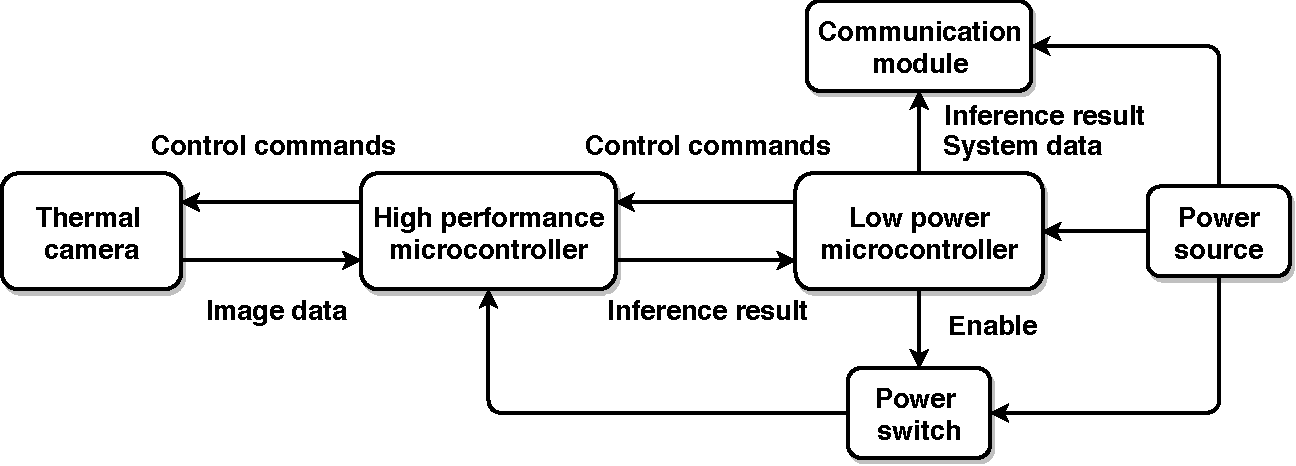
\includegraphics[width=1.0\linewidth]{system_diagram.pdf} 
        \caption{ General block diagram of an embedded system}
        \label{system_diagram}
\end{figure}

The embedded system consists of two different microcontrollers with two distinct tasks, a thermal camera, PIR sensor, wireless communication module, power switch and battery.

Powerful, high-performance microcontroller and thermal camera are usually turned off, to conserve battery life.
A less capable, but low-power microcontroller spends most of the time in low-power mode, waiting for a wakeup trigger from the PIR sensor.
The PIR sensor points in the same direction as the thermal camera and detects any IR radiation of a passing object.

If an object passes PIR's field of vision, PIR sensor produces trigger signal, which consequently wakes up a low power microcontroller.
The microcontroller then enables the power supply to the high-performance microcontroller and thermal camera, and sends a command request for image capture and processing.

The thermal camera only communicates with a high-performance microcontroller, which configures it and requests image data.
That data is then input into a Neural Network algorithm and probability results are then returned to a low power microcontroller.
Low power microcontroller then packs the data and sends it over the radio through a wireless communication module.
The power source to a high-performance microcontroller and thermal camera is then turned off to conserve power.
Diagram of the described procedure can also be seen in Figure \ref{system_flow}.

\begin{figure}[ht]
        \centering
        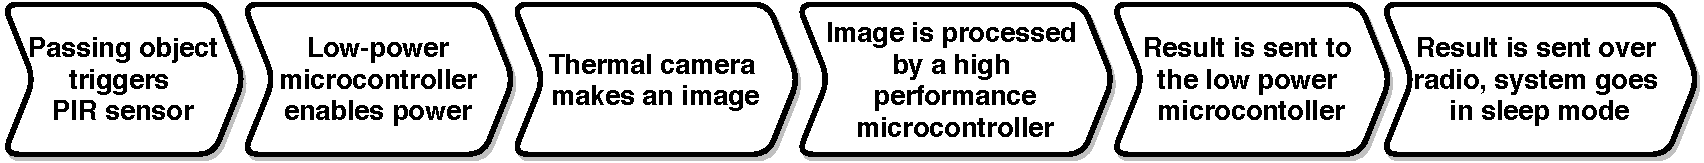
\includegraphics[width=1.0\linewidth]{system_flow.pdf} 
        \caption{ Diagram describing behavior of embedded early warning system} 
        \label{system_flow}
\end{figure}


\section{ Hardware}

In this section, we present concrete components that we used to implement the embedded part of the early warning system.
The hardware version of the embedded system diagram is presented in Figure \ref{hardware_diagram}.
The system consists of various development and evaluation boards.

\begin{figure}[ht]
        \centering
        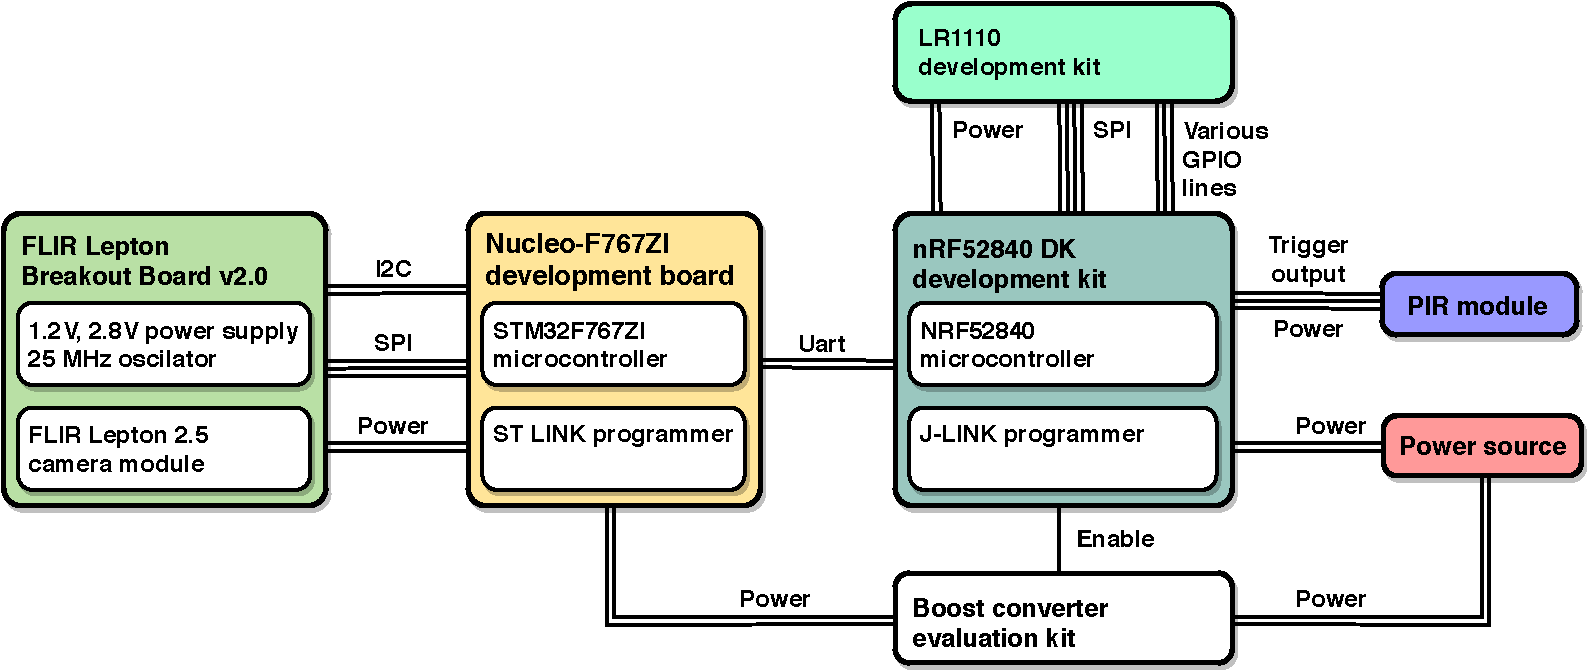
\includegraphics[width=1.0\linewidth]{hardware_diagram.pdf} 
        \caption{ Hardware diagram of embedded early warning system} 
        \label{hardware_diagram}
\end{figure}


\subsection{ Nucleo-F767ZI}

Nucleo-F767ZI (seen on Figure \ref{nucleo}) is a development board made by STMicroelectronics.
Board features STM32F767ZI microcontroller with Cortex-M7 core, which has 2 \si{\mega\byte} of flash, 512 \si{\kilo\byte} of SRAM and can operate at clock speed of 216 \si{\mega\hertz}.
It also features memory caches and a flash accelerator, which provide an extra boost in performance.
It is convenient to program it, as it includes onboard ST-LINK programmer circuit.

\begin{figure}[ht]
        \centering
        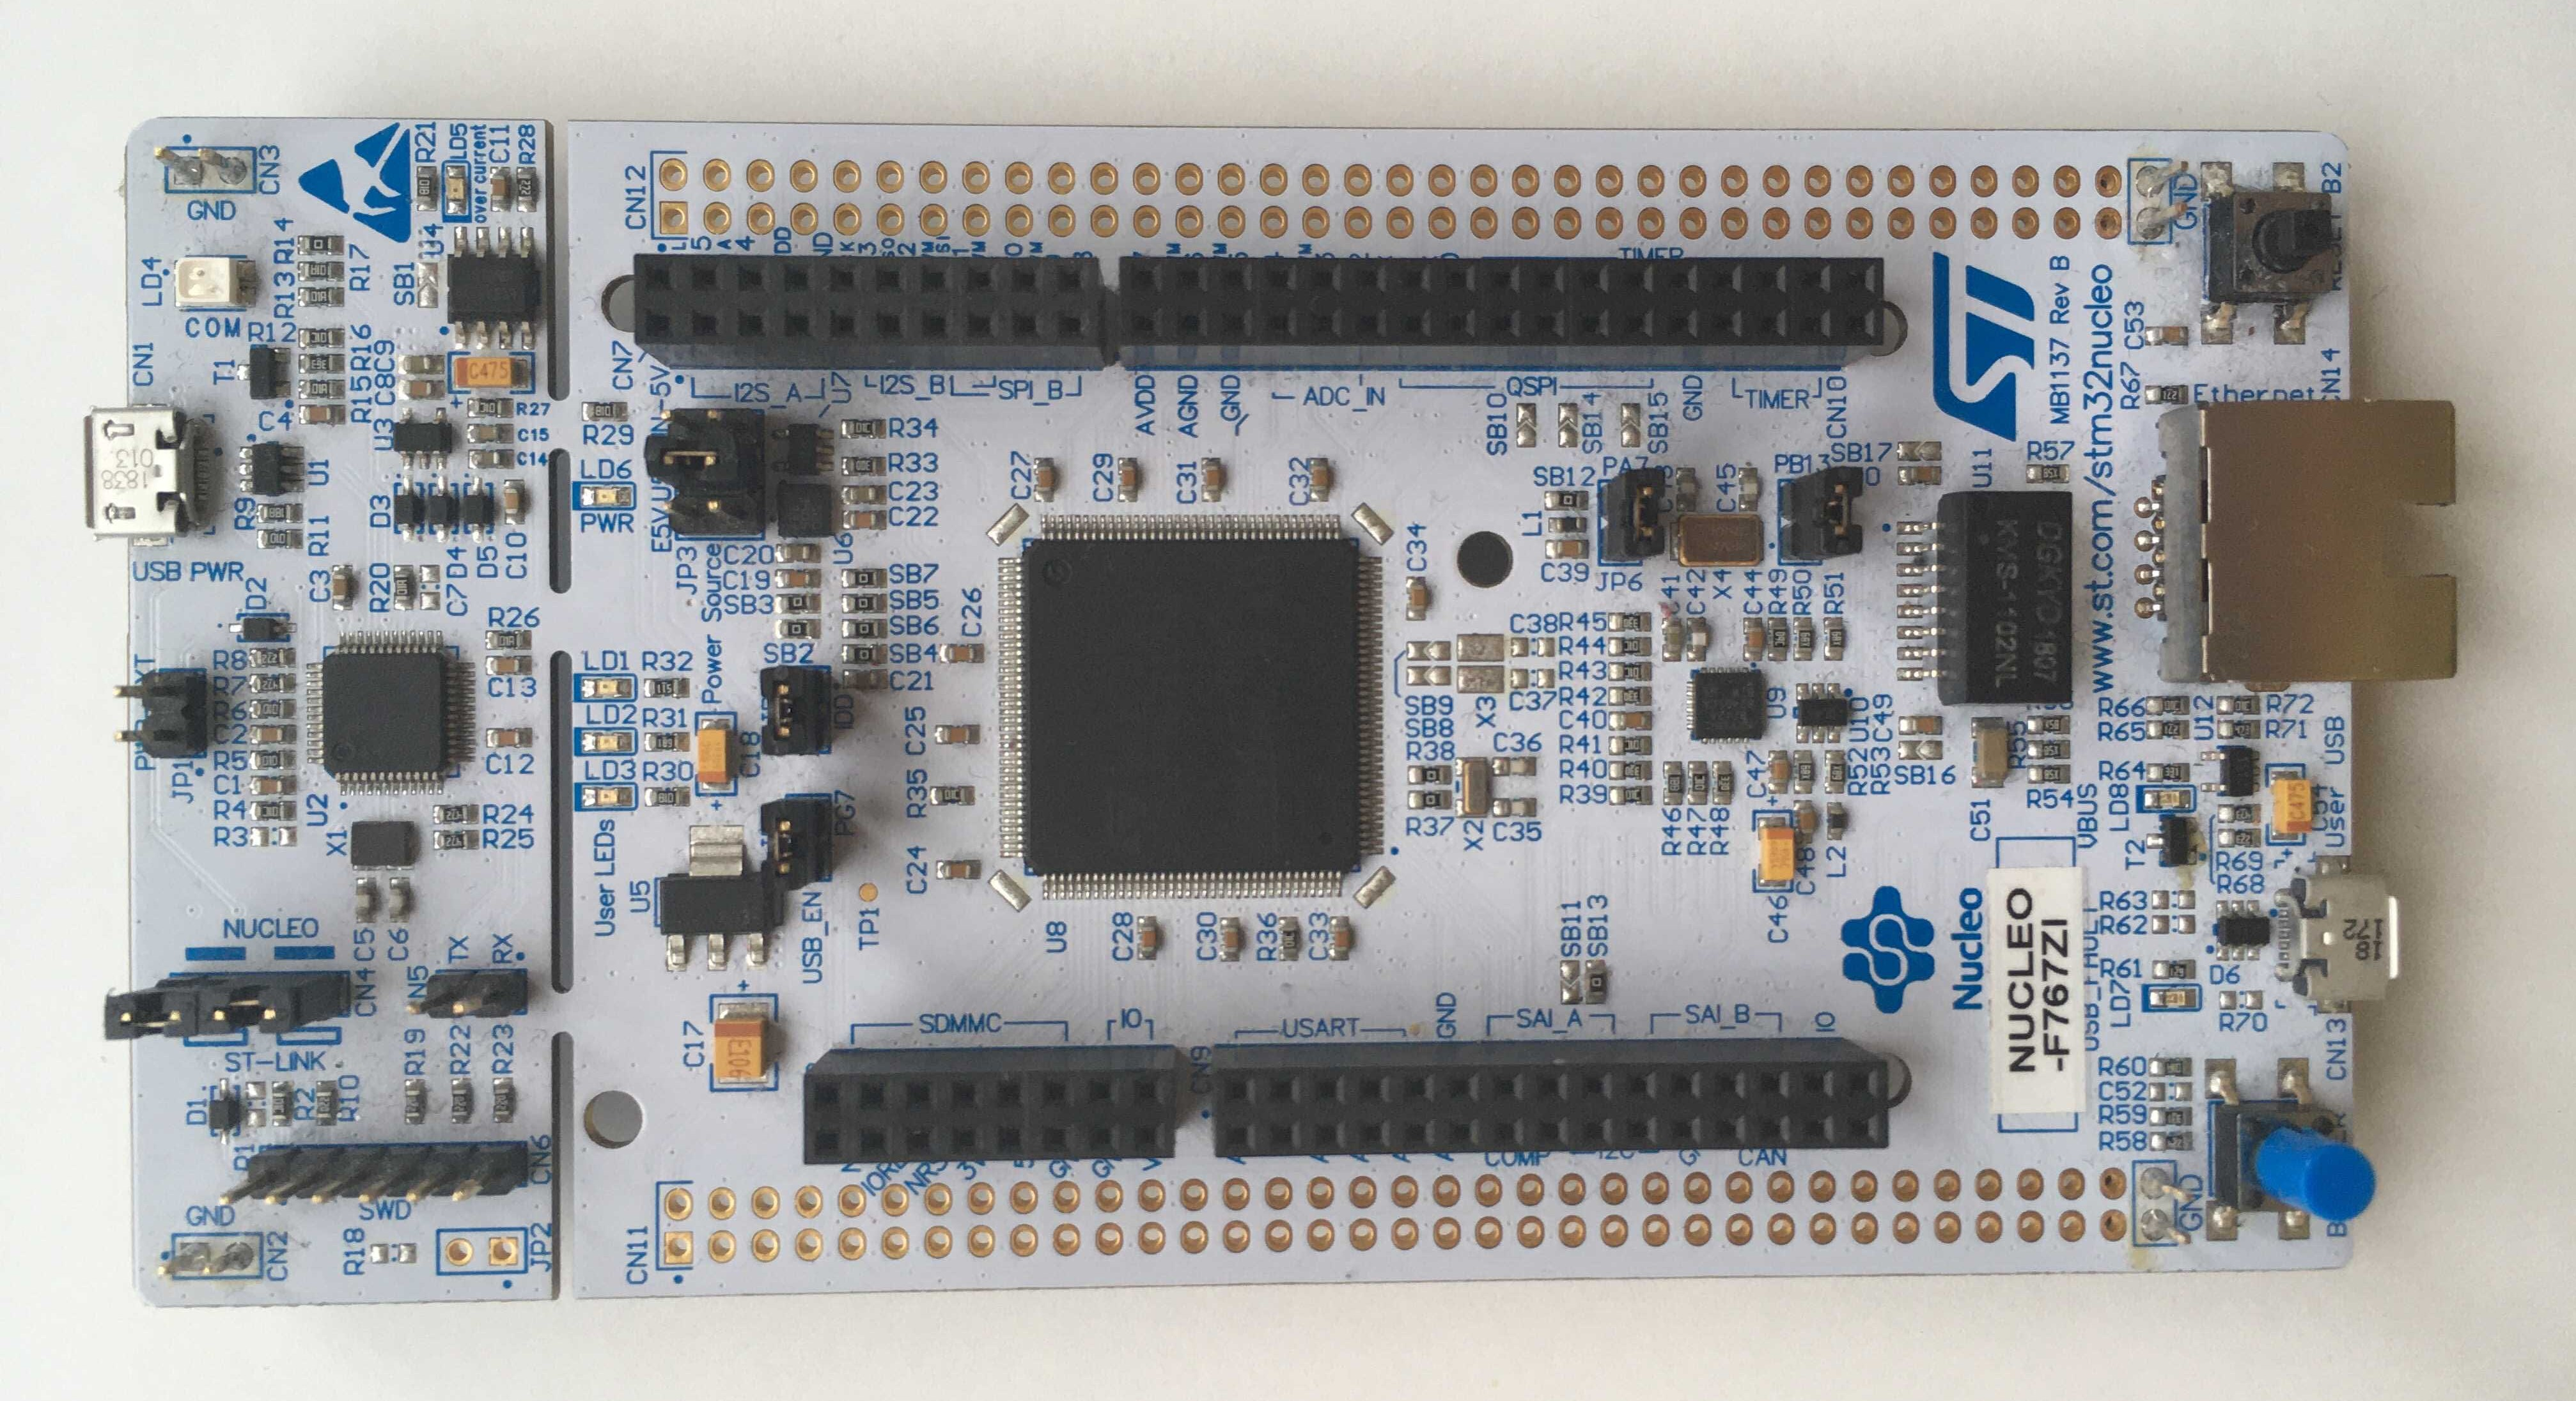
\includegraphics[width=0.75\linewidth]{nucleo.jpg} 
        \caption{ Nucleo-F767ZI development board} 
        \label{nucleo}
\end{figure}

We chose this microcontroller simply because it is one of the more powerful general purpose microcontrollers on the market.
As we knew that Neural Networks are computationally expensive to compute and that models can be quite large in terms of memory, we selected it knowing that we can always scale down, if we have to.


\subsection{ nRF52840 DK}

For the part of the system, which had to contain a low-power microcontroller and would control the communication module and power control for the Nucleo-F767ZI board, we decided to use the nRF52840 development kit.
The development kit, made by Nordic Semiconductor, can be seen in Figure \ref{nrf_board}

The main logic on the board is provided by an nRF52840 microcontroller with Cortex-M4 core, which has 1 \si{\mega\byte} of flash, 256 \si{\kilo\byte} of RAM and a Bluetooth 5 support.
nRF52840 has a consumption of 0.5 \si{\micro\ampere} in sleep mode, which makes it ideal for our purpose.

\begin{figure}[ht]
        \centering
        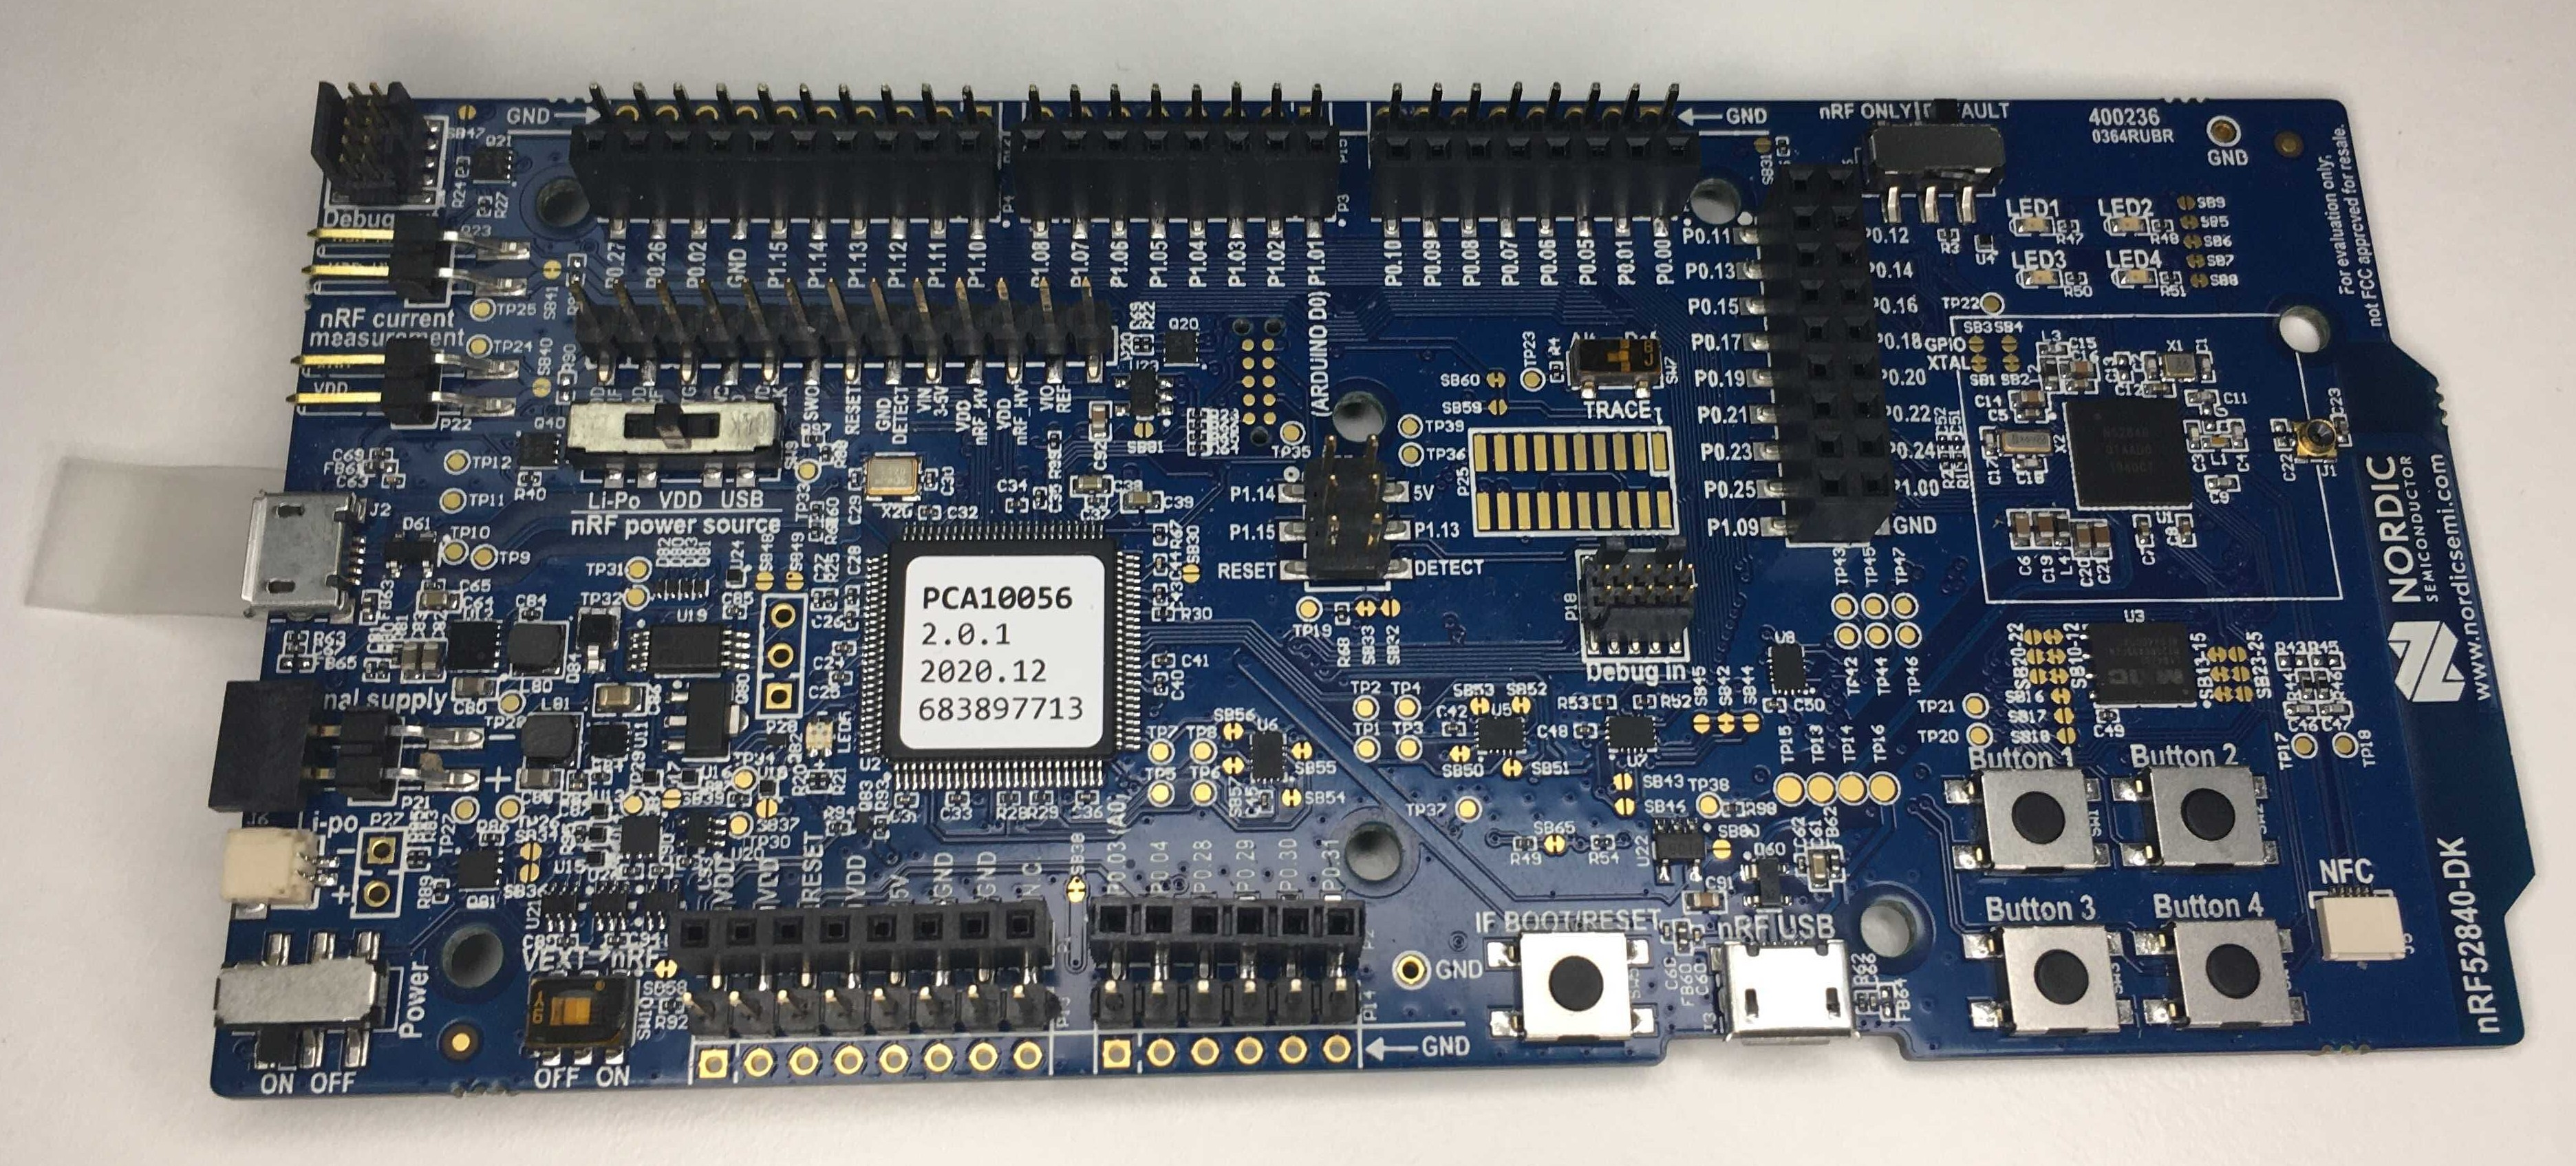
\includegraphics[width=0.75\linewidth]{nrf_board.jpg} 
        \caption{ nRF52840DK development board}
        \label{nrf_board}
\end{figure}

\subsection{ LR1110 development kit}

For the role of the LoRa transceiver module, we decided to use Semtech's development kit which uses the LR1110 chip.
LR1110 is a multi-functional solution as it contains LoRa transceiver, GNSS and WiFi geoposition scanning modules.
Development kit seen in Figure \ref{lr1110_board} contains an LR1110 chip, three different antennas and its respective tuning networks.
It comes in a convenient Arduino shield form factor, which means that we can directly attach it to nRF52840 DK without any jumper wires.

\begin{figure}[ht]
        \centering
        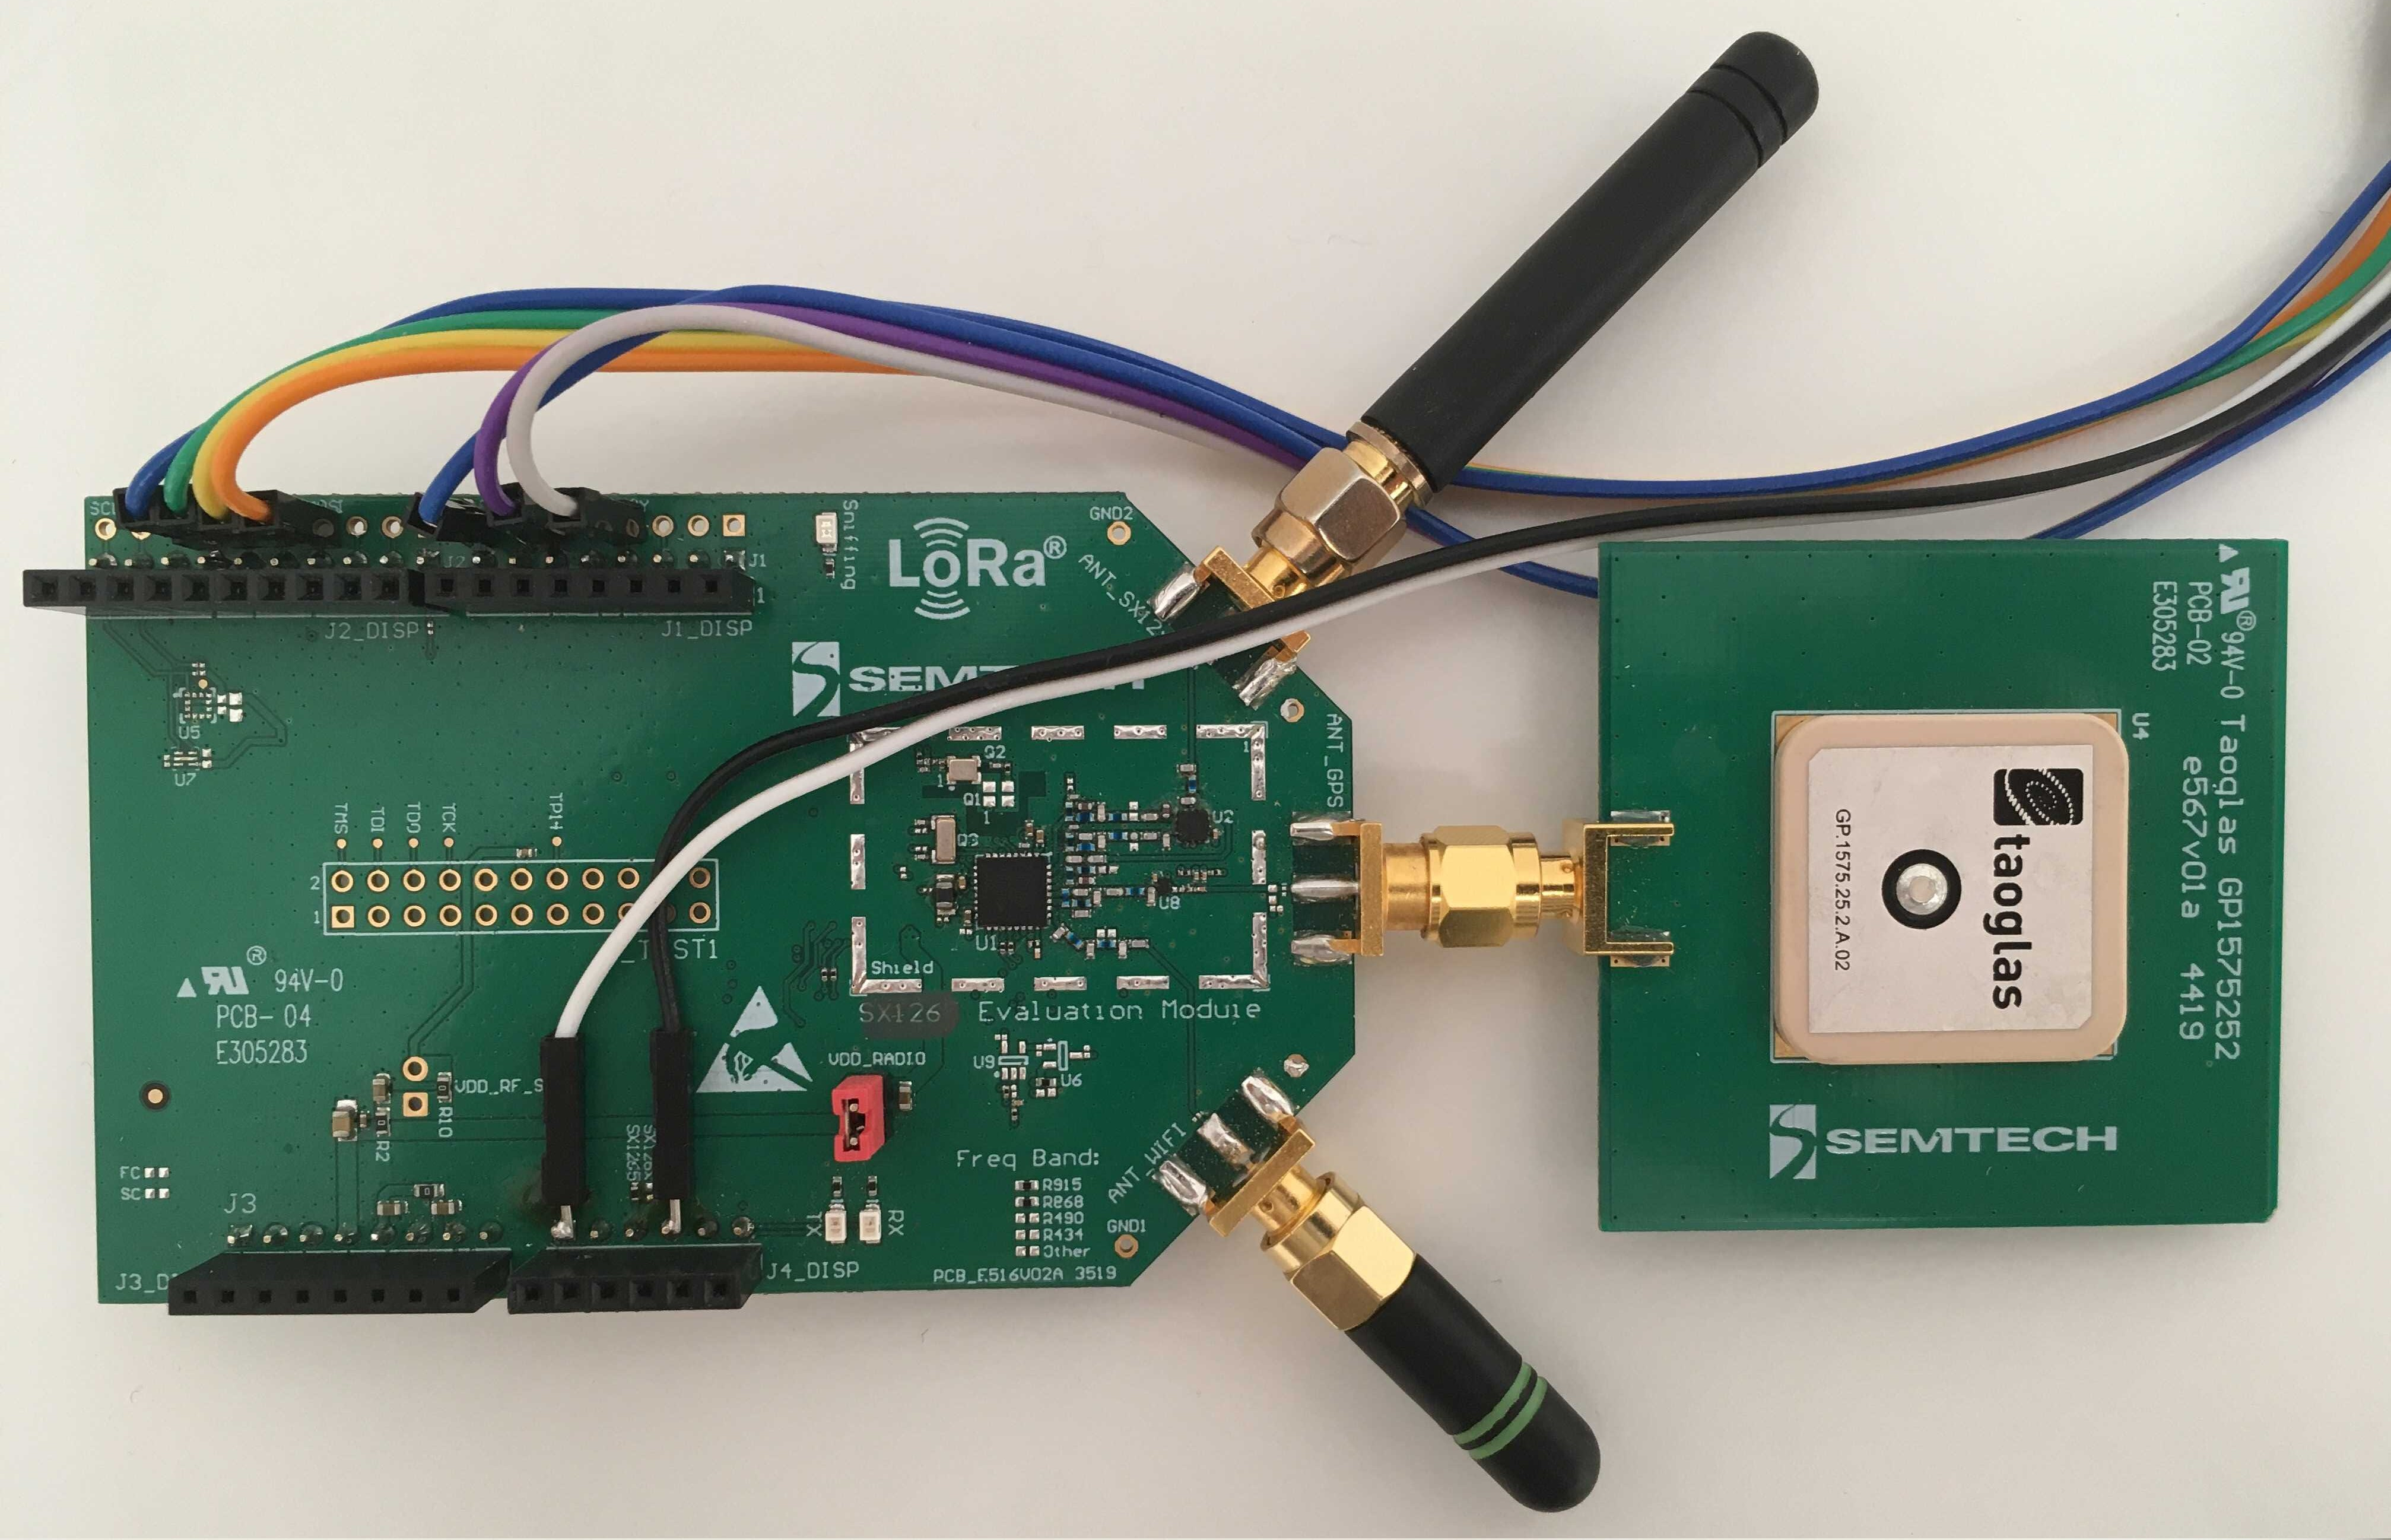
\includegraphics[width=0.75\linewidth]{lr1110_board.jpg} 
        \caption{ MAX17225ENT+T boost converter breakout board}
        \label{lr1110_board}
\end{figure}

\subsection{ Boost converter evaluation kit}

Power control of the Nucleo-F767ZI board and the FLIR camera is provided by the MAX17225ENT+T boost converter chip.
Breakout board containing the chip is shown in Figure \ref{boost_converter}.
Operating the boost converter chip is simple, its enable line can be directly connected to a microcontroller pin, driving it high will enables output and driving it low disables it.
The output voltage is controlled by an external resistor.

\begin{figure}[ht]
        \centering
        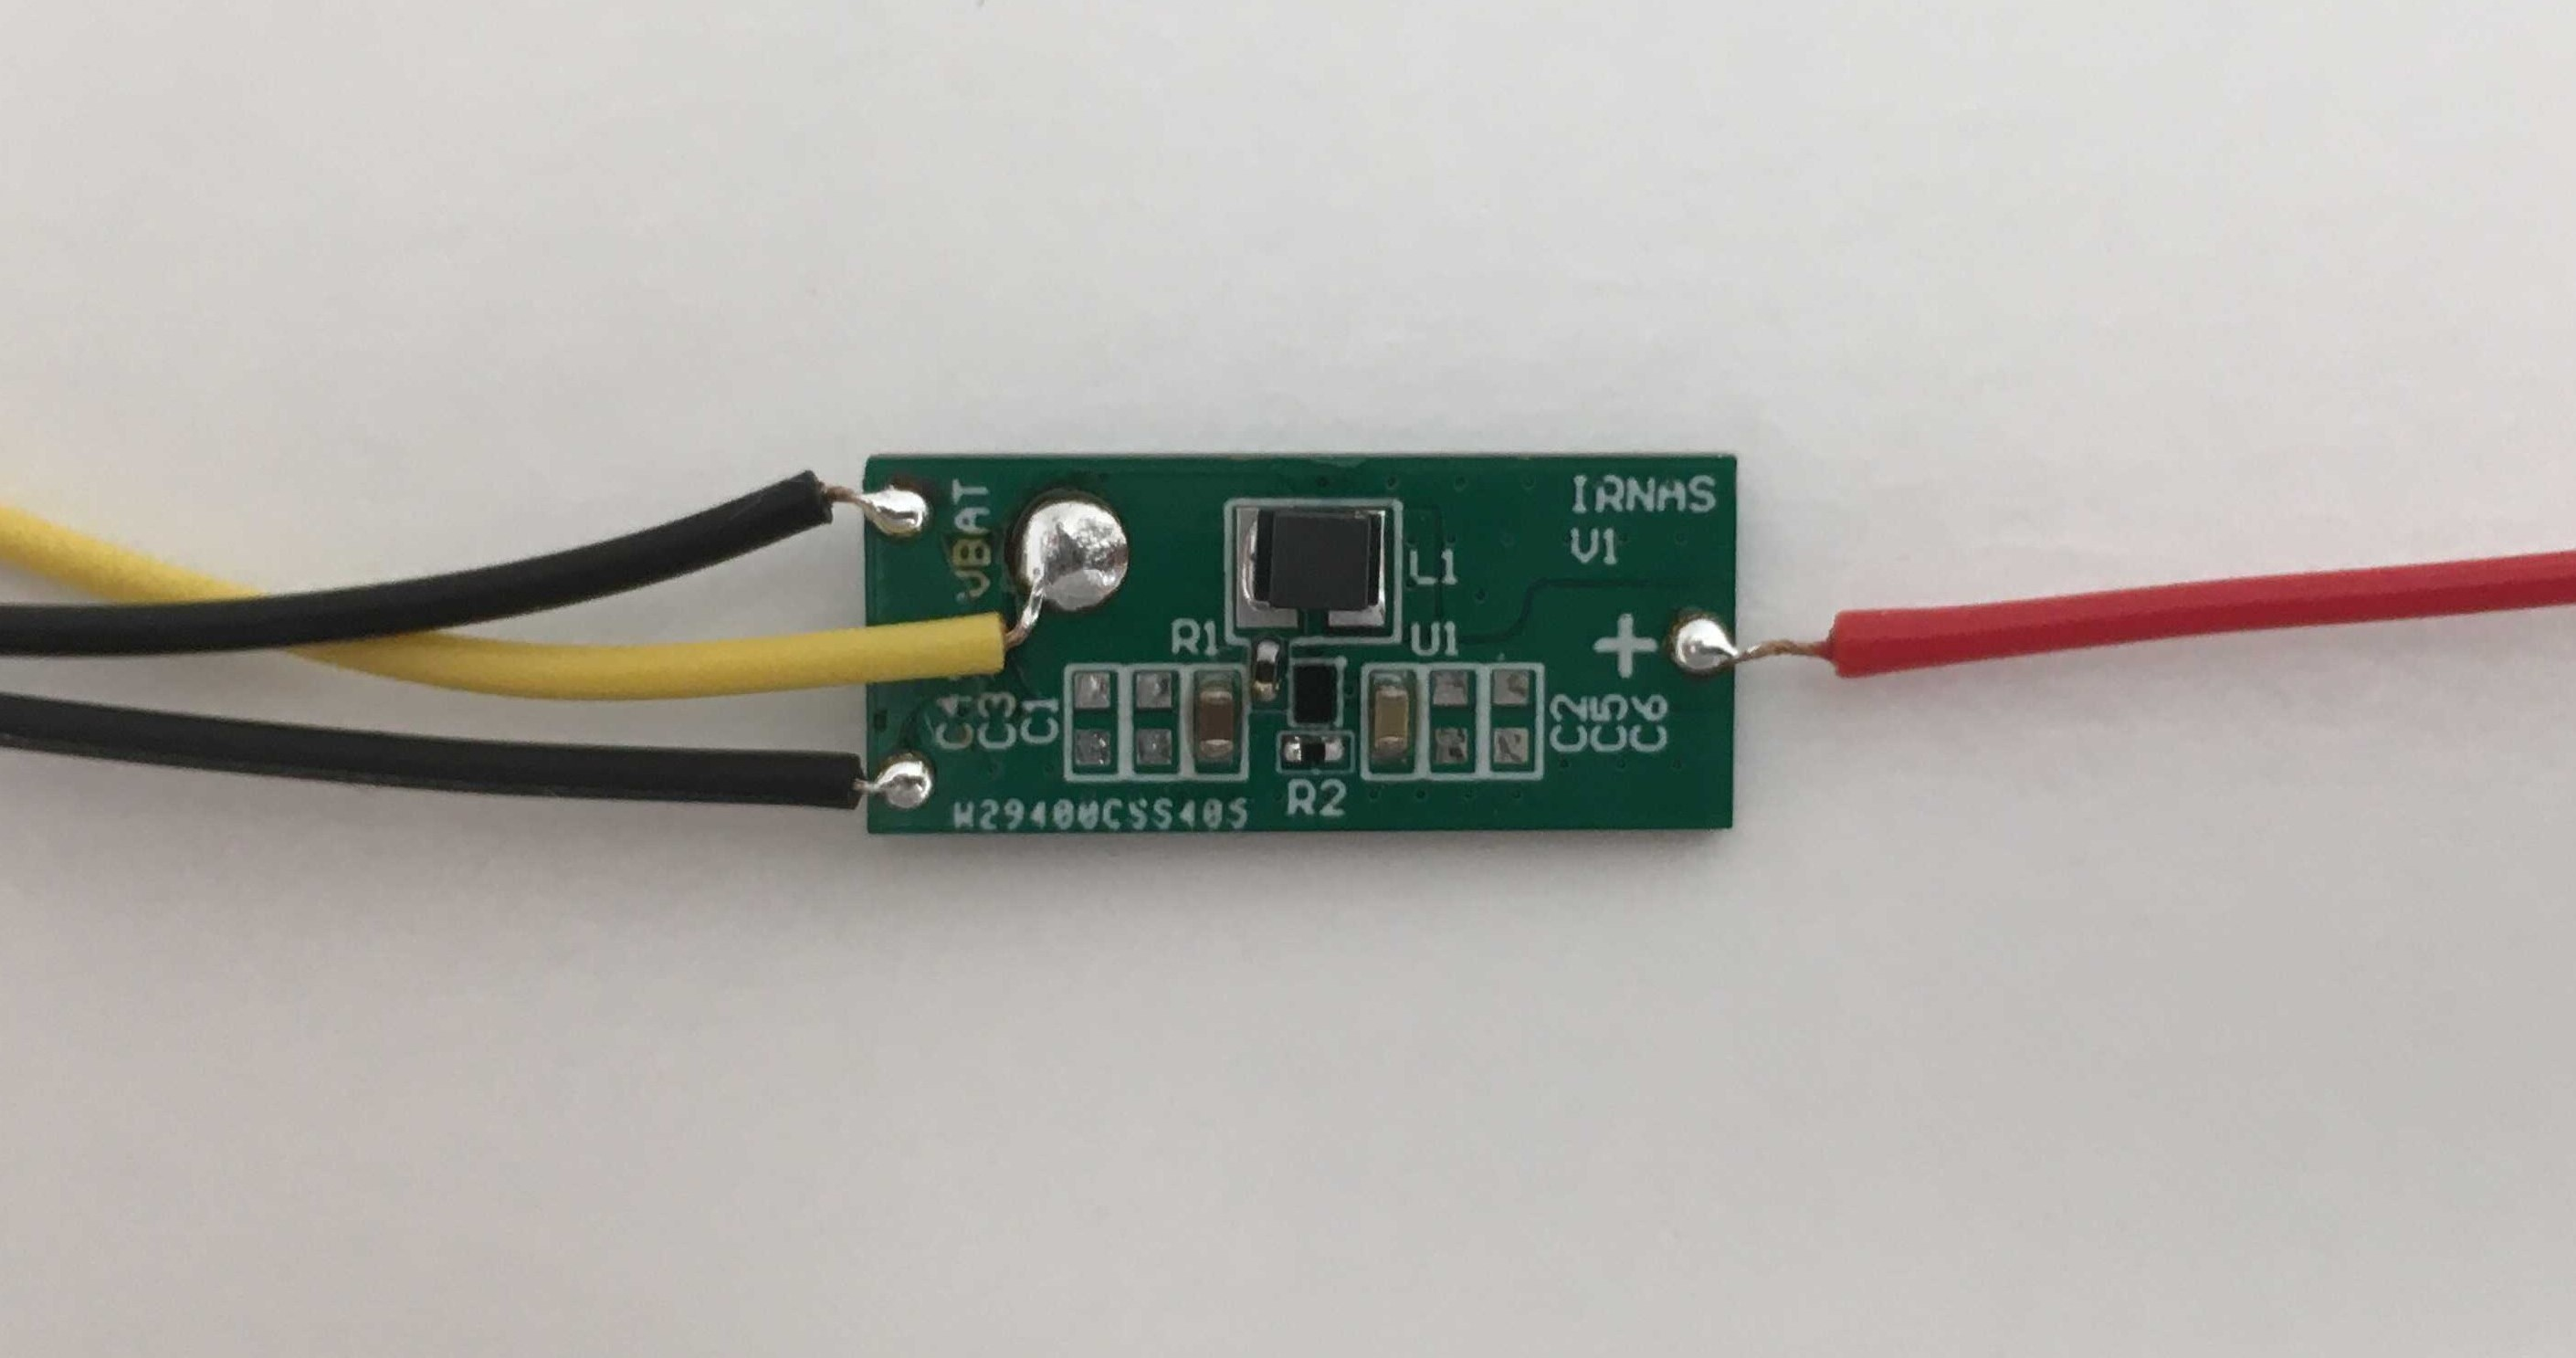
\includegraphics[width=0.75\linewidth]{boost_converter.jpg} 
        \caption{ MAX17225ENT+T boost converter breakout board}
        \label{boost_converter}
\end{figure}

\subsection{ FLIR Lepton 2.5 camera module and Lepton breakout board}

Section \ref{thermal_cameras} described what kinds of thermal cameras exist and how do they work, and Section \ref{choosing_thermal} described why FLIR Lepton 2.5 was chosen.
However, not much was said about what sort of support circuitry FLIR camera needs and how do we make images with it.

FLIR Lepton camera is powered from two different sources, 1.2 \si{\volt} and 2.8 \si{\volt}, and requires a reference clock of 25 \si{\mega\hertz}.
All of this is provided by the Lepton breakout board, which can be seen in Figure \ref{lepton_breakout}.
The front side of the breakout board contains a FLIR module socket and the backside contains two voltage regulators and an oscillator.
Breakout board can be powered from 3.3 to 5 \si{\volt} and also conveniently breaks out all communication pins in form of header pins.

\begin{figure}[ht] 
    \begin{subfigure}[b]{0.5\textwidth}
        \centering
        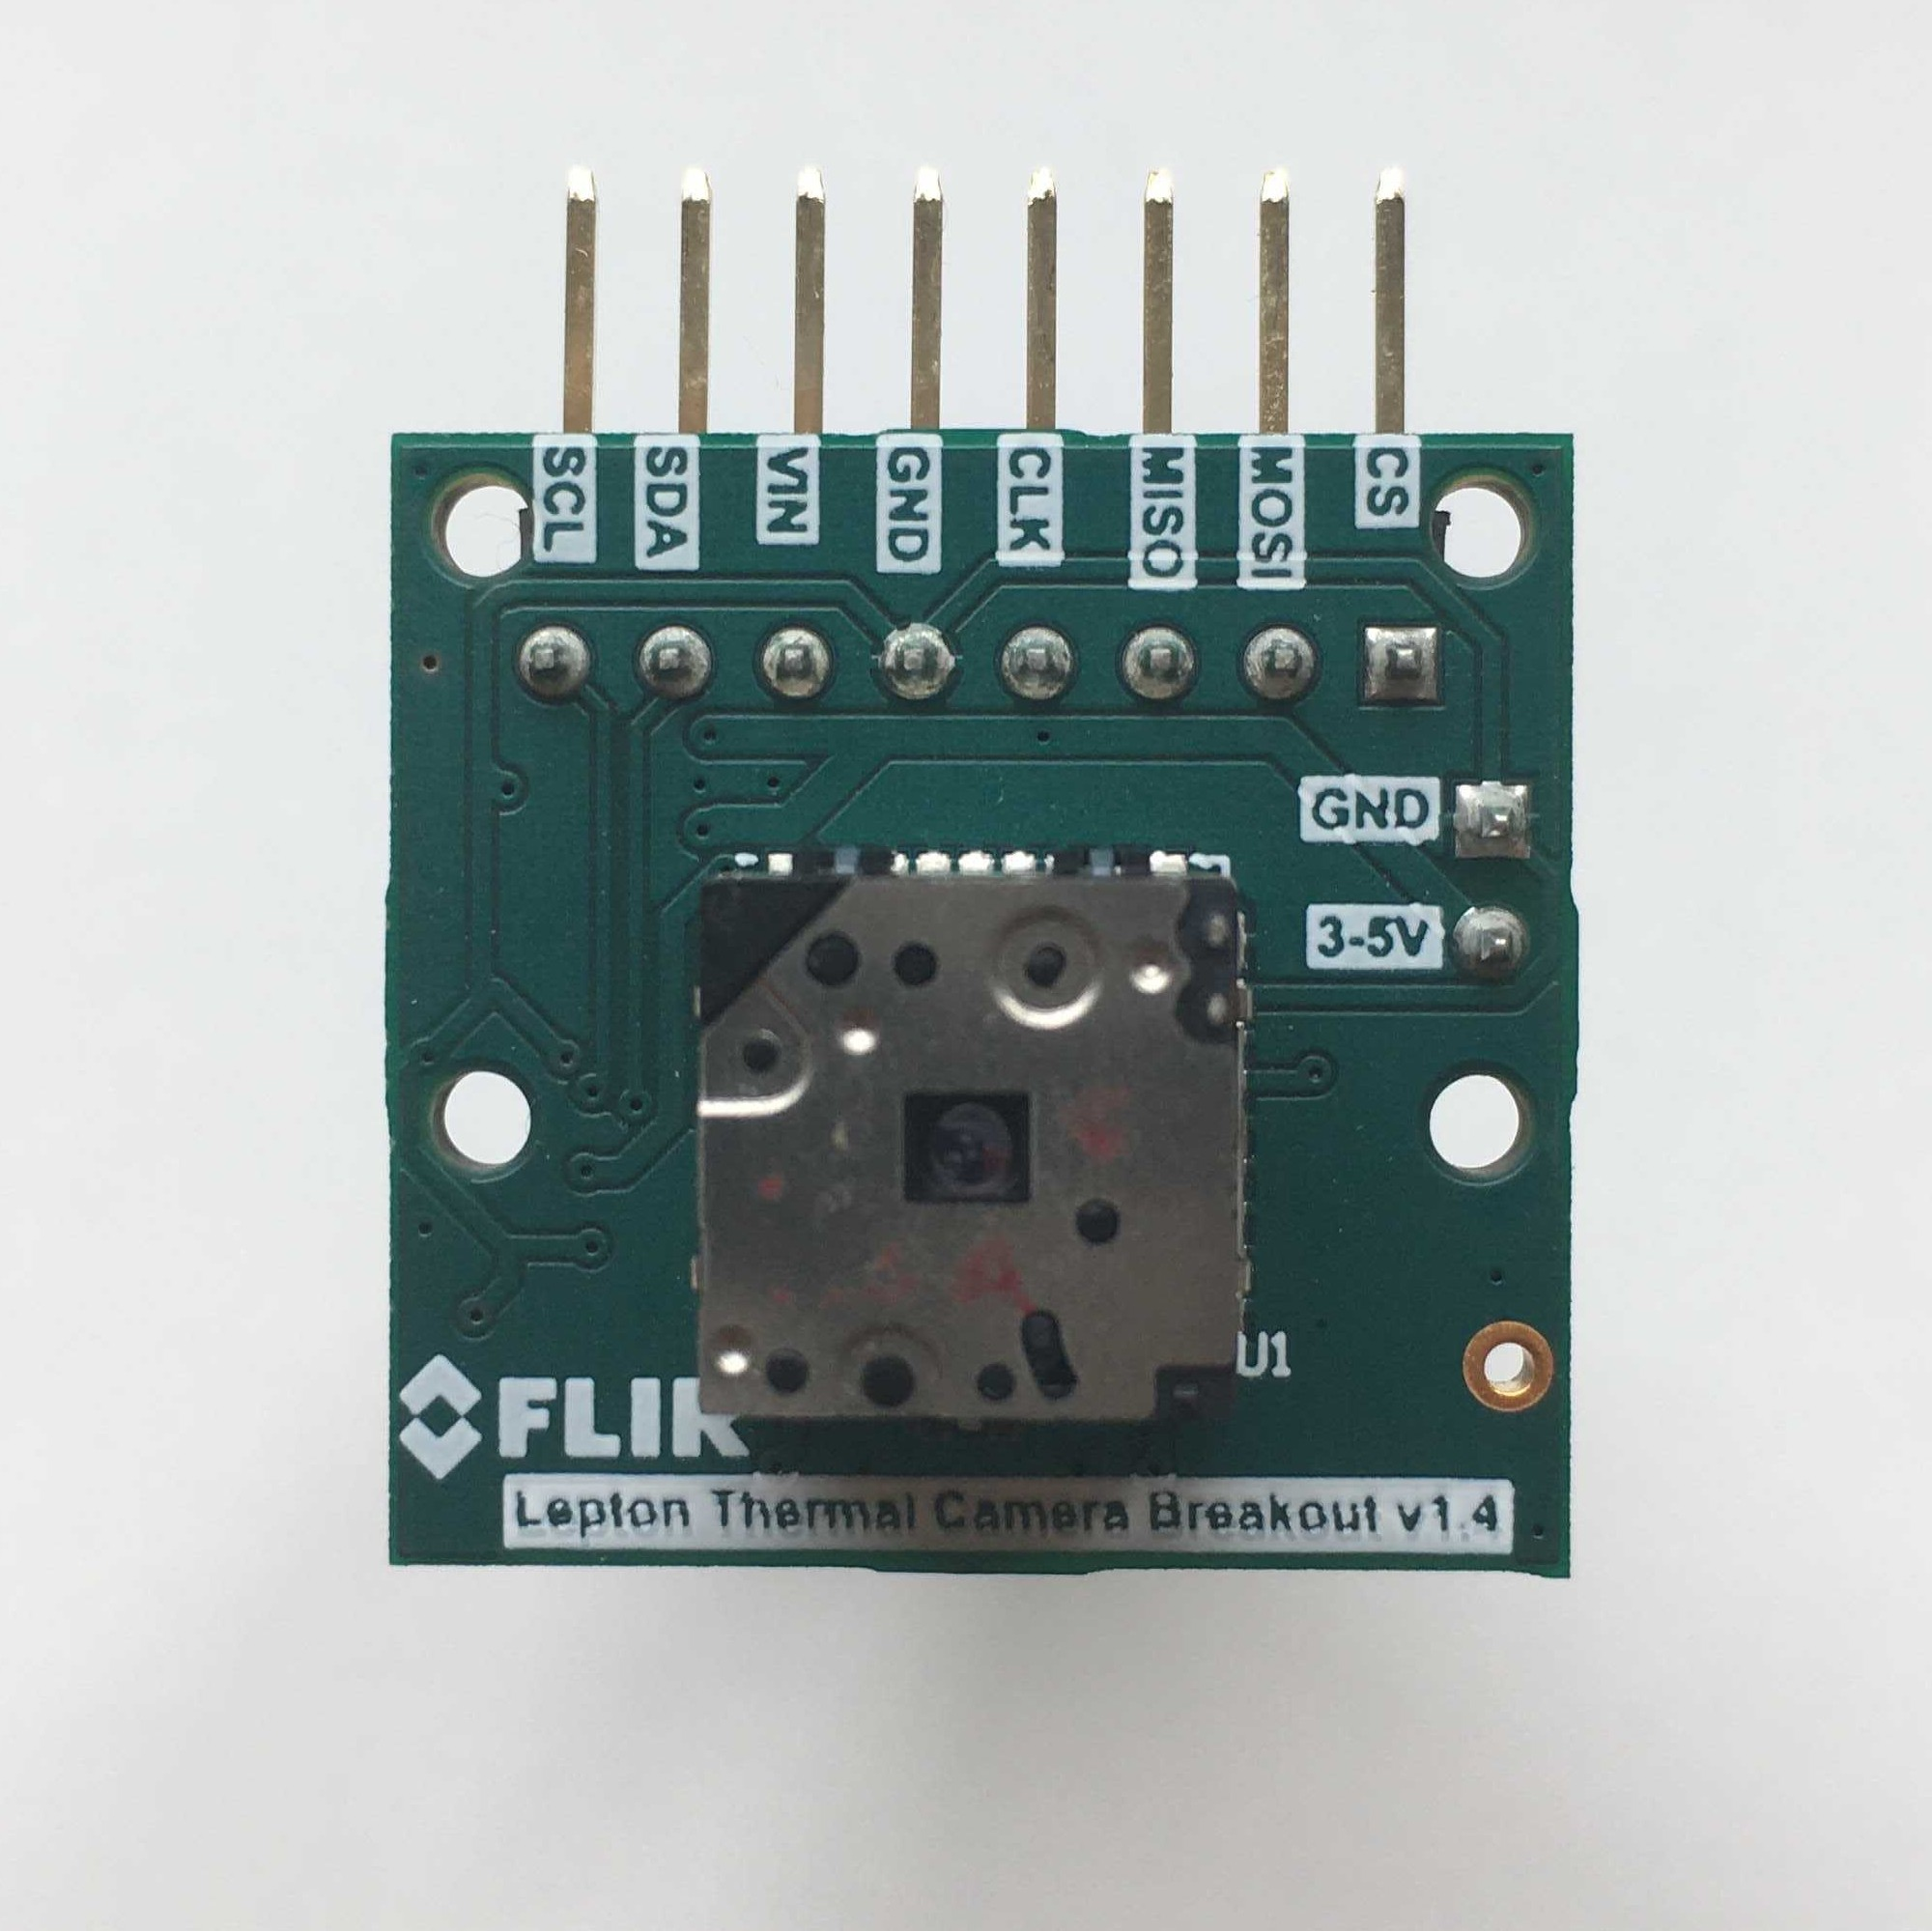
\includegraphics[width=1.0\linewidth]{flir_module_front.jpg} 
    \end{subfigure}
    \begin{subfigure}[b]{0.5\textwidth}
        \centering
        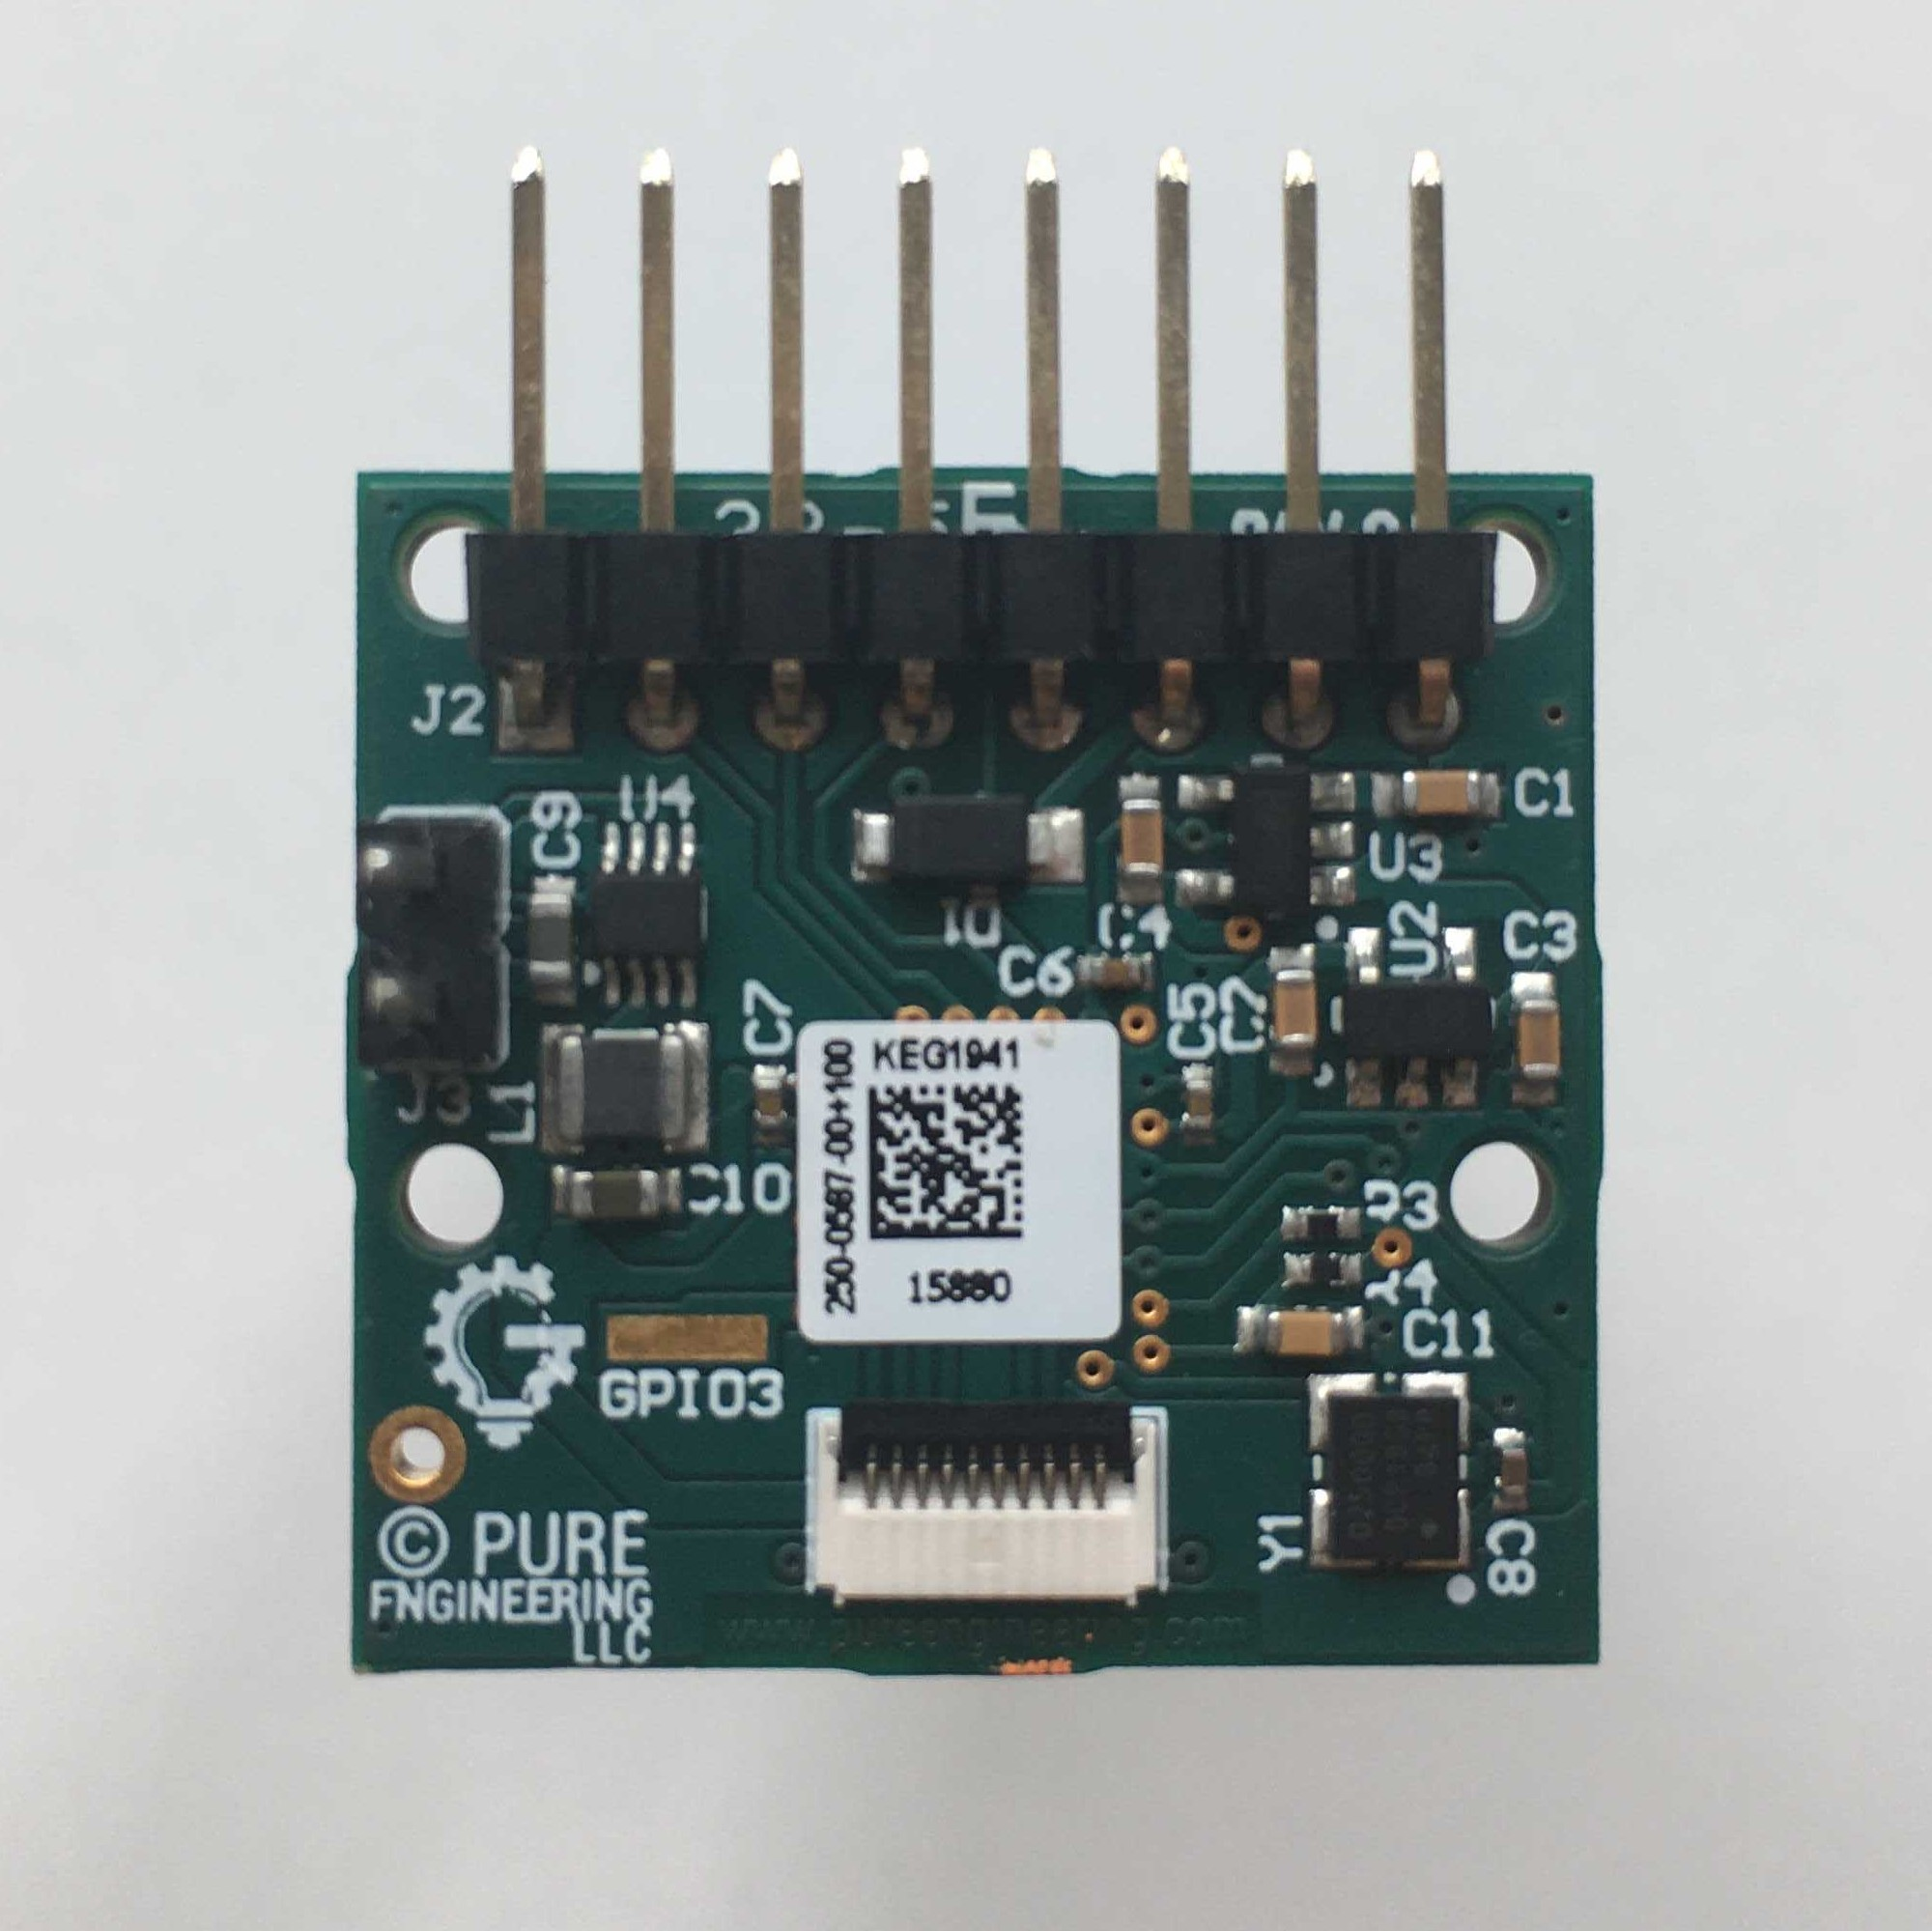
\includegraphics[width=1.0\linewidth]{flir_module_back.jpg} 
    \end{subfigure}
    \caption{ Front and back side of FLIR Lepton breakout board with thermal camera module inserted.}
    \label{lepton_breakout}
\end{figure}

FLIR Lepton module itself contains five different subsystems that work together and can be configured:

\begin{itemize}
    \item AGC – Automatic Gain Control, affects image contrast and quality
    \item SYS – System Information
    \item VID – Video Processing Control
    \item OEM – Camera configuration for OEM customers
    \item RAD – Radiometry
\end{itemize}

Task of AGC subsystem is to convert a dynamic range of an IR sensor into a compact range that is more suitable for storing and displaying images.
In the case of FLIR Lepton, this is a 14-bit to 8-bit conversion.
For our purposes, the AGC subsystem was turned on, as the input to our image classification model were 8-bit values.

The microcontroller communicates with FLIR camera over two interfaces: two-wire interface (TWI) is used for control of the FLIR camera and Lepton's VoSPI protocol is used for image transfer.

TWI is a variation of an I2C protocol, instead of 8 bits all transfers are 16 bits.
The internal structure of the Lepton's control block can be seen in Figure \ref{flir_lepton_cci}.
Whenever we are communicating with the FLIR camera we have to specify which subsystem are we addressing, what type of action we want to do (get, set or run), length of data and data itself.

\begin{figure}[ht]
        \centering
        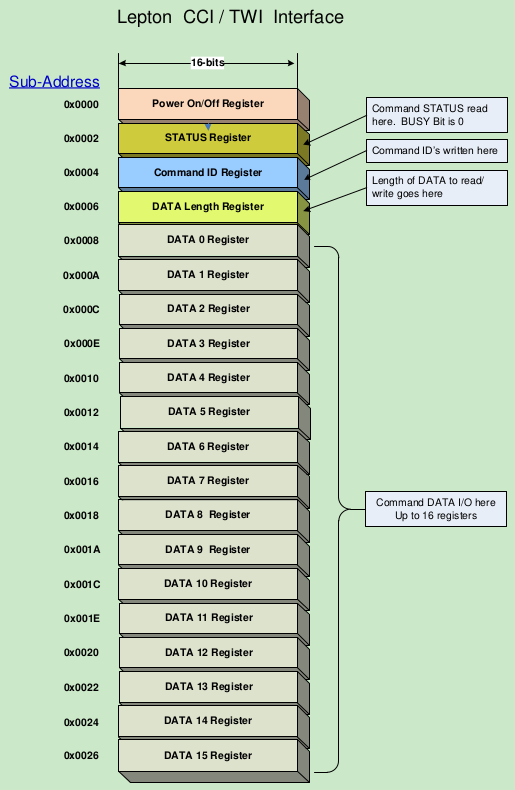
\includegraphics[height=12cm]{flir_lepton_cci.png} 
        \caption{ Command and control interface of FLIR Lepton camera.} 
        \label{flir_lepton_cci}
\end{figure}

Lepton's VoSPI protocol is used only to stream image data from the camera module to the microcontroller, which means that the MOSI line is not used.
Each image fits into one VoSPI frame and each frame consists of 60 VoSPI packets.
One VoSPI packet contains 2 bytes of an ID field, 2 bytes of a CRC field and 160 bytes of data\footnotemark, which represents one image line.

The refresh rate of VoSPI frames is 27 \si{\hertz}, however, only every third frame is unique from the last one.
It is the job of the microcontroller to control the SPI clock speed and process each frame fast enough so that the each unique frame is not discarded.
\footnotetext{ Because images pixel values fit into the 14-bit range by default, it means that one-pixel value needs two bytes of data (two most significant bytes are zero). That means that each image line (80 pixels) is stored in 160 bytes. If AGC conversion is turned on, each pixel is then mapped into an 8-bit range, however, the size of one line in the VoSPI packet remains 160 bytes, 8 most significant bits are simply zeros.}
\subsection{ PIR Sensor}

We used a cheap, generic PIR sensor, that can be seen in Figure \ref{pir_sensor}.
It has two potentiometers, which are used to adjust sensor's sensitivity and detection delay.
PIR sensor runs on 3.3 V, which enables us to directly power it from the nRF52840 DK. 

\begin{figure}[ht] 
    \begin{subfigure}[b]{0.5\textwidth}
        \centering
        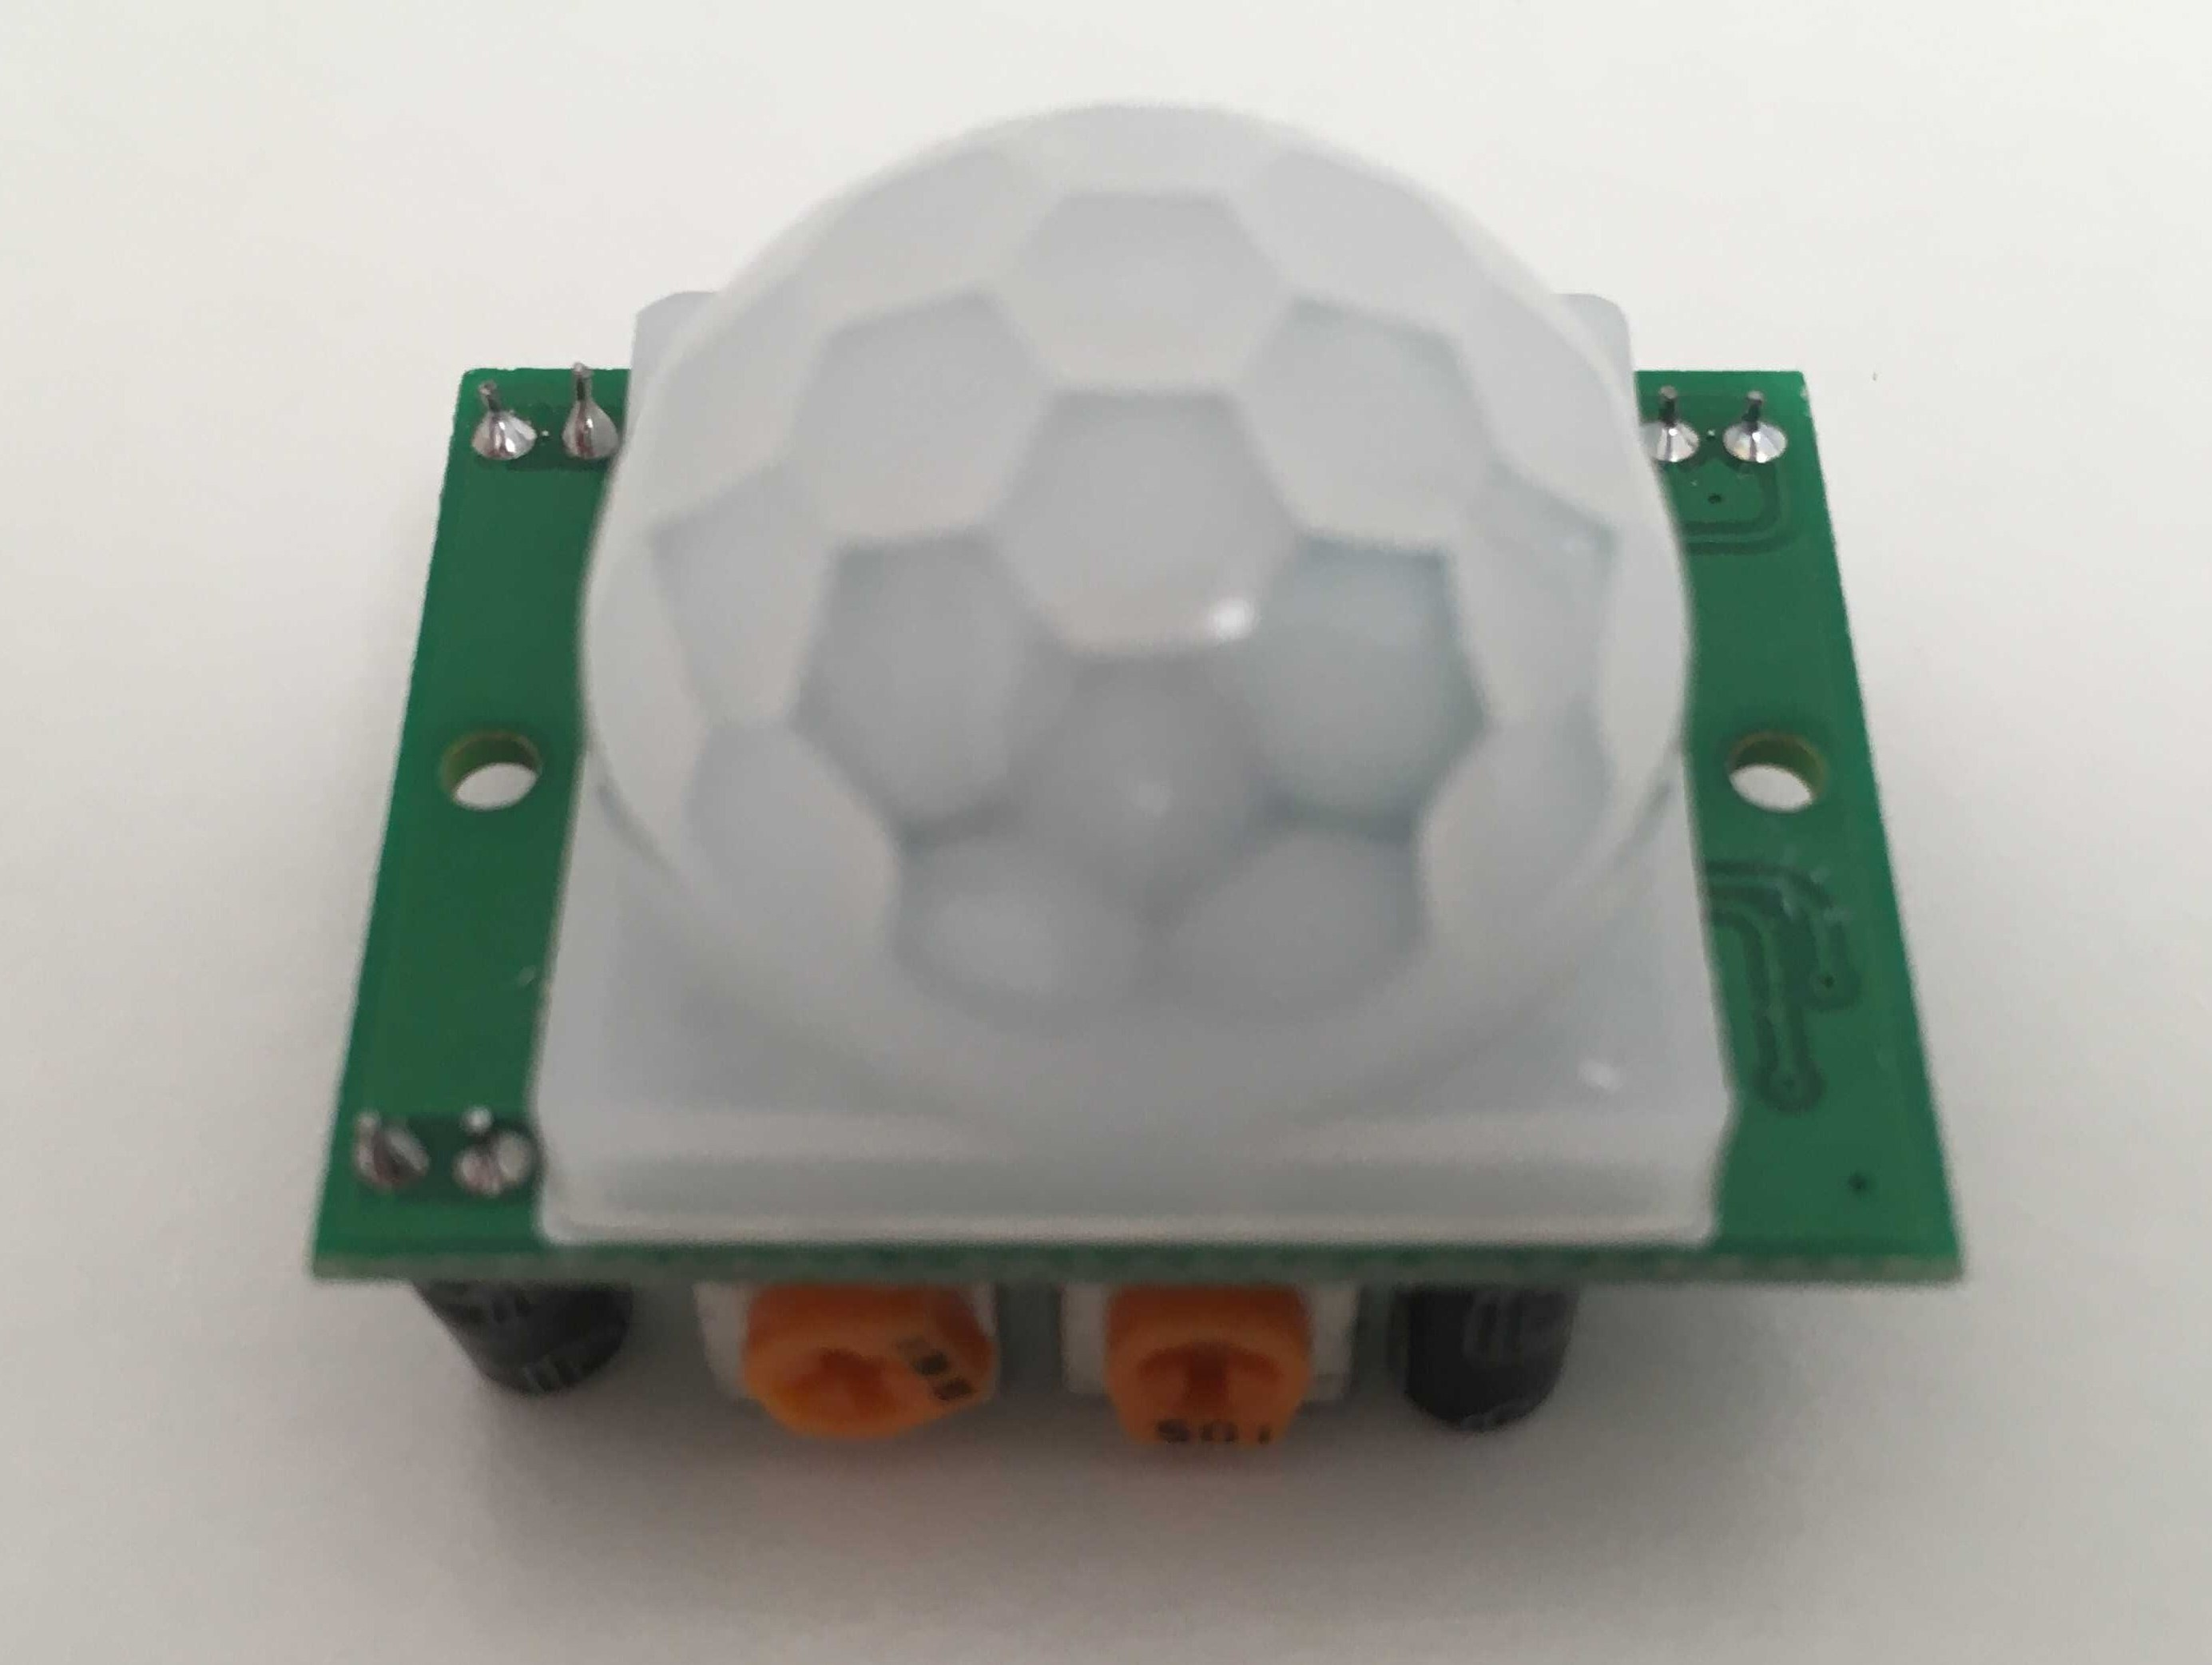
\includegraphics[width=1.0\linewidth]{pir_top.jpg} 
    \end{subfigure}
    \begin{subfigure}[b]{0.5\textwidth}
        \centering
        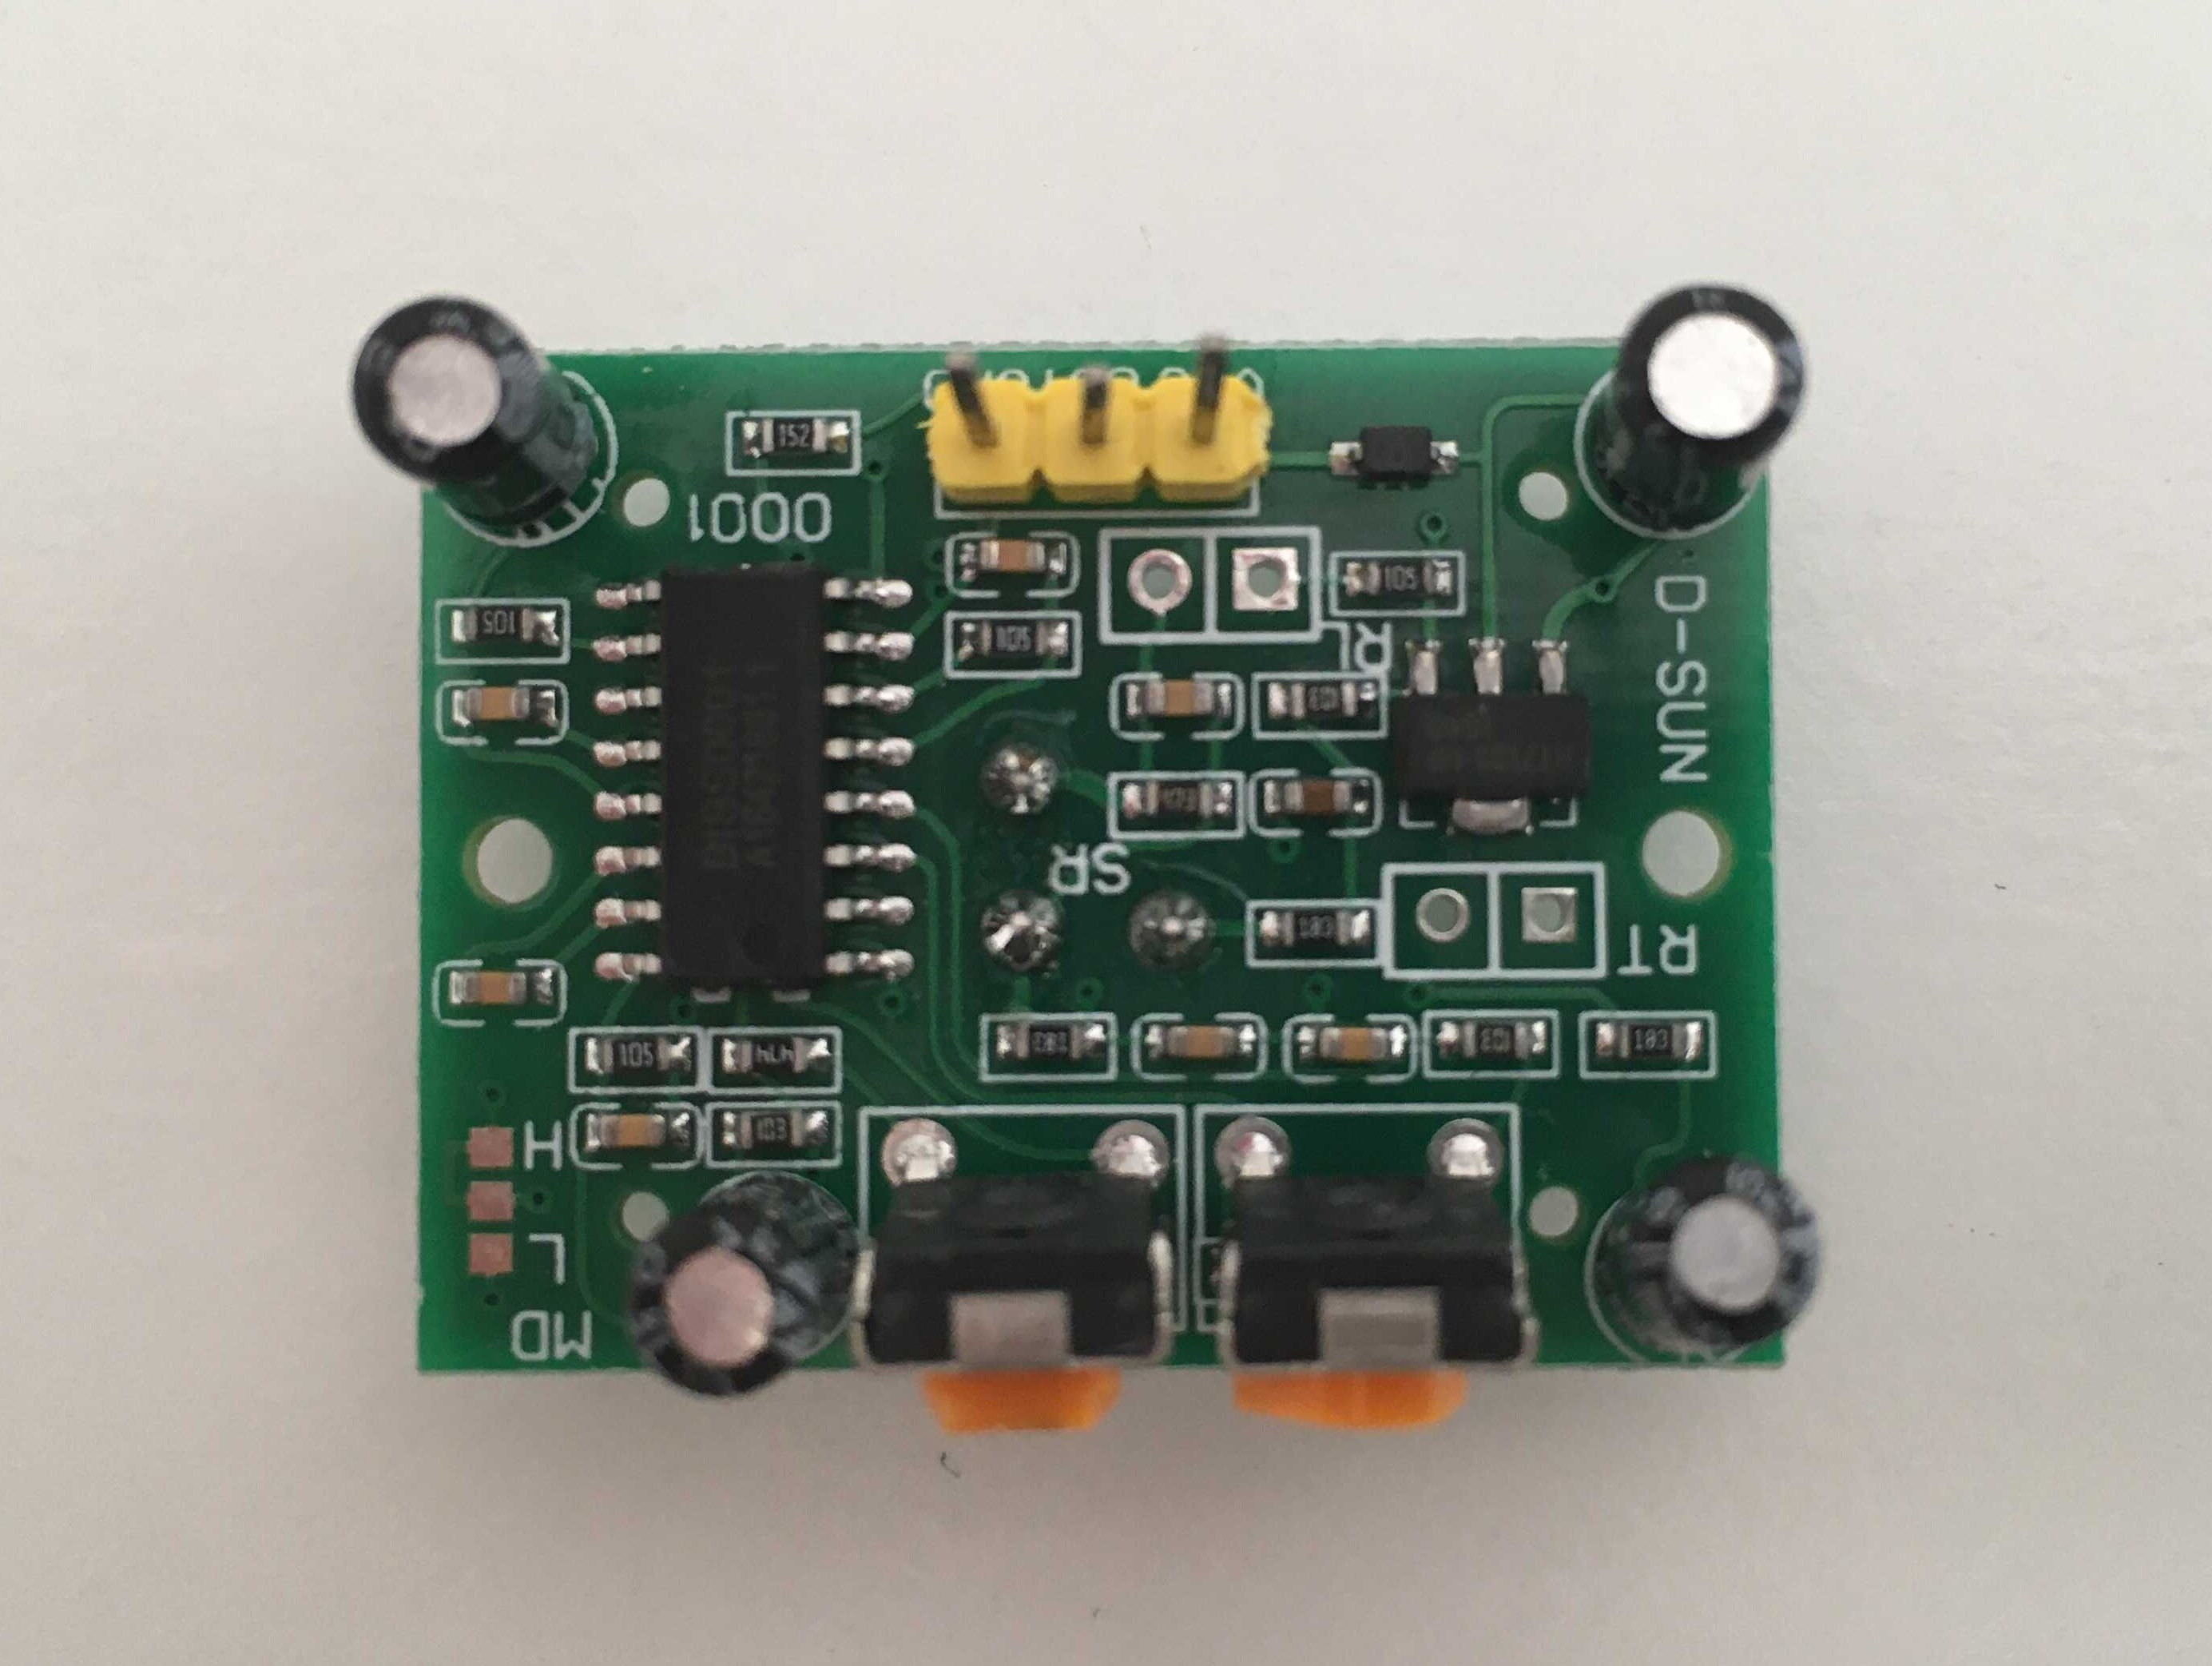
\includegraphics[width=1.0\linewidth]{pir_bot.jpg} 
    \end{subfigure}
    \caption{ Front and back side of FLIR Lepton breakout board with thermal camera module inserted.}
    \label{pir_sensor}
\end{figure}

\section{ Firmware}
\subsection{ Tools and development environment}

For our firmware development we did not choose any of the integrated development environments, provided by different vendors.
Instead we used terminal text editor Vim for writing and editing the code.

As we were programming two different microcontrollers, we were using different tools for each one.


\subsubsection{ Development environment for STM32f767ZI}

For building our firmware programs we used GNU Make, build automation that builds software according to user written \textit{Makefiles}.
To compile code we used the Arm embedded version of GNU GCC.
To program binaries into our microcontroller we used OpenOCD.

For hardware abstraction library we used libopencm3, which is an open-source low-level library that supports many of Arm's Cortex-M processors cores, which can be found in a variety of microcontroller families such as ST's STM32, Toshiba's TX03, Atmel's SAM3U, NXP's LPC1000, Silabs's EFM32 and others.
Libopencm3 provided us with linker files, startup routines, thinly wrapped peripheral drivers and a starting template makefile, which served as a starting point for our project.

As libopencm3 does not provide \verb|printf| functionality out of the box we used an excellent library by GitHub user mpaland\cite{printf_lib}.


\subsubsection{ Development environment for nRF52840}

To develop firmware for nRF52840 we decided to use The Zephyr OS, which is a small kernel, designed for IoT embedded systems.
Besides usual RTOS functionalities such as tasks, mutexes, semaphores it also provides a common driver API for supported microcontrollers.


\subsection{ Architecture design}

STM32F767ZI firmware was designed to be very efficient and lean, only truly necessary parts of firmware were implemented.

As seen in Figure \ref{firmware_diagram} we split the firmware into two hardware and application modules.

\begin{figure}[ht]
        \centering
        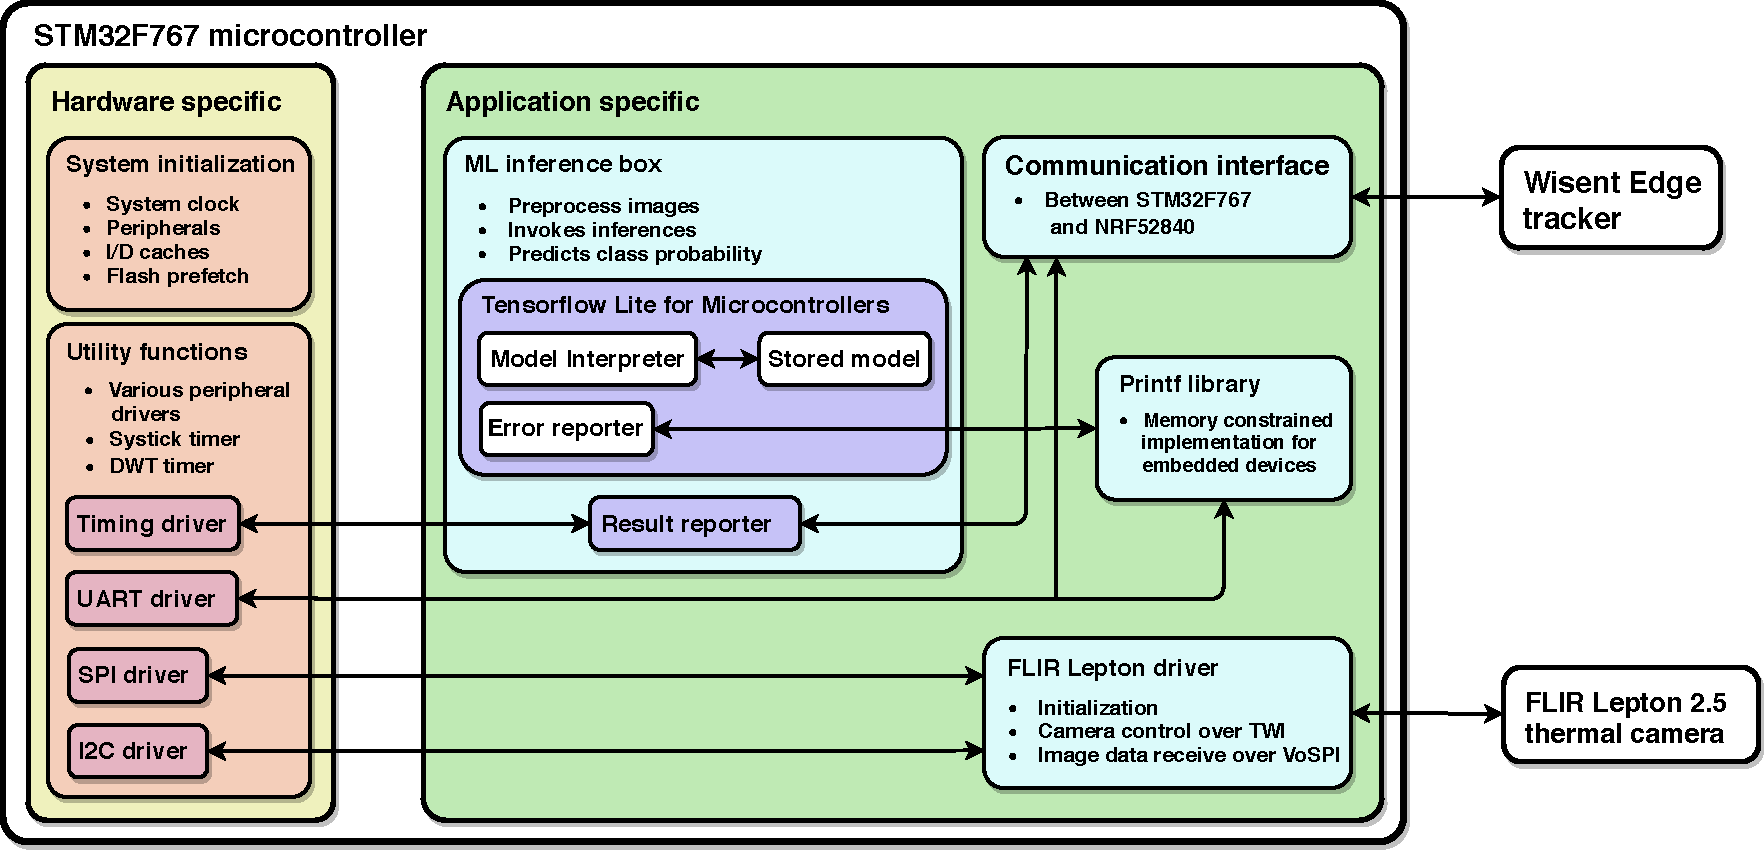
\includegraphics[width=1.0\linewidth]{firmware_diagram.pdf} 
        \caption{ Architecture diagram of the firmware that is running on a STM32F767ZI microcontroller.} 
        \label{firmware_diagram}
\end{figure}

Hardware specific module is mostly using libopencm3 API to set the system clock and initialize peripherals.
Small function wrappers had to be written to make use of various peripheral drivers easier.

FLIR Lepton driver was written from scratch, as many libraries provided either by the camera manufacturer or open source communities were too complex and implemented many features that we did not require.

Thanks to TFLite Micro API, the ML inference module could be written as a simple black box.
Image data goes in, predictions come out.

The architecture diagram for nRF52840 can be seen on Figure \ref{firmware_diagram_wisent}.
For the nRF52840 microcontroller we did not had to write any peripheral drivers, as they were provided by Zephyr itself.

\begin{figure}[ht]
        \centering
        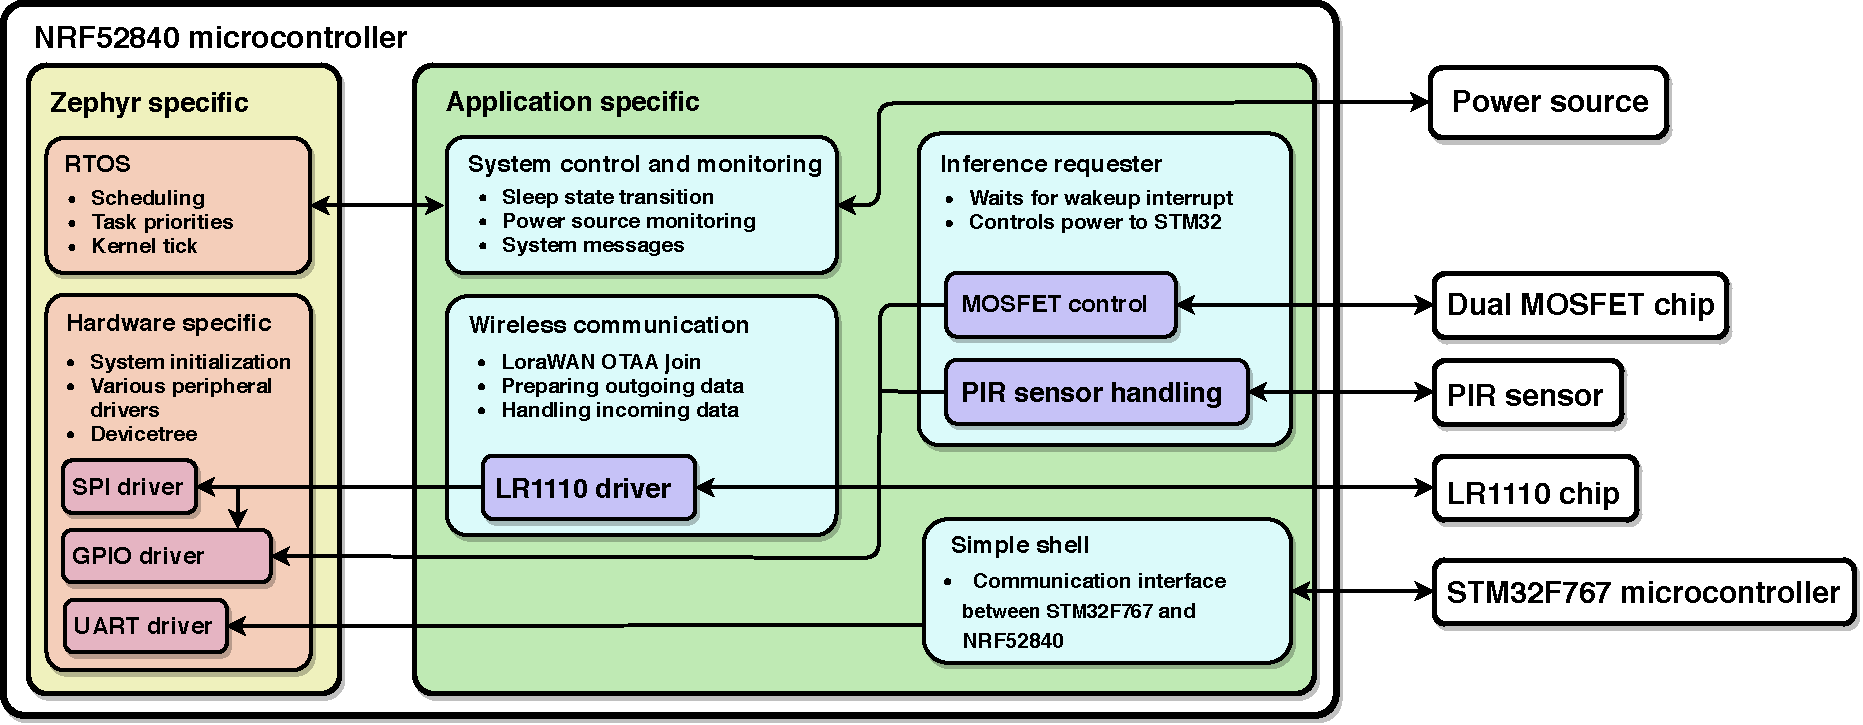
\includegraphics[width=1.0\linewidth]{firmware_diagram_nrf.pdf} 
        \caption{ Architecture diagram of the firmware that is running on a nRF52840 microcontroller.} 
        \label{firmware_diagram_wisent}
\end{figure}

Utmost importance was achieving low power consumption.
That meant that nRF52840 had to spend most of its time in low-power mode, only waking up for regular system checks and PIR trigger signals.
When PIR trigger signal would be received, the interrupt would wake up the nRF52840, which would then enable a boost converter, thus enabling power to STM32F67 and FLIR Lepton camera.

For the communication interface, we decided to implement a simple UART shell module.
nRF52840 microcontroller would act as a host and send commands to STM32F767ZI.
STM32F767ZI would execute commands and send back results.
Such setup enabled us to test each microcontroller separately.

Once we knew that UART communication worked correctly, we could issue commands directly from the computer's serial port, which enabled us to develop and test firmware for STM32F767ZI separately from nRF52840 firmware.

We also wrote a communication module, which takes care of controlling the LR1110 chip, joining the LoRaWAN network, preparing outgoing messages and sending them over the LoRaWAN network.


\subsection{ MicroML and build system} \label{build_system_label}

A large part of this thesis was concerned with porting TFLite Micro to libopencm3, our platform of choice.
To understand how this could be done, we first had to analyse how the code is built in TFLite Micro.

To compile source files and build binaries TFLite Micro uses GNU Make.
The main makefile includes several platform specific makefiles, which dictate how firmware is built, and several bash scripts which download various dependencies.
By providing command-line arguments users decide which example needs to be compiled and for which platform.
The build system makes some assumptions about locations of the platform specific files, which in case of example projects are scattered over the whole TensorFlow GitHub repository.

We learned a useful principle while analysing the build process. 
Each time we would build an example for a new platform, Make would first compile all TensorFlow files, create a static library out of them, compile specific example source files and then link against the library in linking stage.
If we wanted to build firmware for a different example, but for the same platform, Make would only have to compile source files of that example and link them with previously made library.
As compilation of required TensorFlow files takes quite some time, this was an efficient option.

After analysing the TFLite Micro's build system we created a list of requirements that we wanted to fulfil on our platform.

\begin{enumerate}
    \item We wanted to keep project-specific code, libopencm3 code and TFLite Micro code separated.
    \item We wanted a system, where it would be easy to change a microcontroller specific part of a building process.
    \item We wanted to reuse static library principle that we saw in TFLite Micro build process.
\end{enumerate}

Covering different platforms and use cases made main TFLite Micro makefile quite complex and hard to understand.
This meant that it would be hard to reuse it while porting to a new platform and we needed a different approach or reuse something else.

To solve our problem we started developing a small project that we named MicroML\footnotemark.
MicroML enables users to develop ML applications on microcontrollers supported by libopencm3.
Project's directory structure can be seen in Figure \ref{microml_dir}

\footnotetext{ Project is open-source and publicly available on GitHub\cite{microml}.}

\begin{figure}[ht] 
    \centering
    \begin{minipage}{7cm}
    \dirtree{%
    .1 MicroML.
    .2 tensorflow.
    .2 libopencm3.
    .2 projects.
    .3 hello\_world\_stm32f7.
    .3 elephant\_stm32f7.
    .4 test.
    .4 src.
    .4 Makefile.
    .4 project.mk.
    .4 openocd.cfg.
    .2 archive\_makefile.
    .2 rules.mk.
    }
    \end{minipage}
    \caption{ Directory structure of MicroML project.}
    \label{microml_dir}
\end{figure}

Folders \verb|tensorflow| and \verb|libopencm| are directly cloned from their respective sources as Git submodules, which means that they are fixed at specific commits, usually at major release points.
In folder \verb|projects| users place all their specific projects.
Besides source files, each project has to contain three specific files:

\begin{itemize}
    \item \textbf{project.mk} - It contains information which files need to be compiled inside the project folder. In it is defined for which microcontroller the code needs to be compiled and what kind of optimisation flags should be used.
    \item \textbf{openocd.cfg} - Configuration file that tells OpenOCD which programmer interface needs to be used to flash a microcontroller and the location of the binary file that needs to be flashed.
    \item \textbf{Makefile} - Project's makefile that gathers source files inside the project folder. It makes it possible to call \verb|make| directly from projects directory, which eases the development process. It does not specify any building rules, those are specified in included \verb|rules.mk| file in the root directory of the project.
\end{itemize}

Some initial commands need to be executed when the project is cloned from the GitHub for the first time. 
Figure \ref{build_system} represents the complete build process.

\begin{figure}[ht]
        \centering
        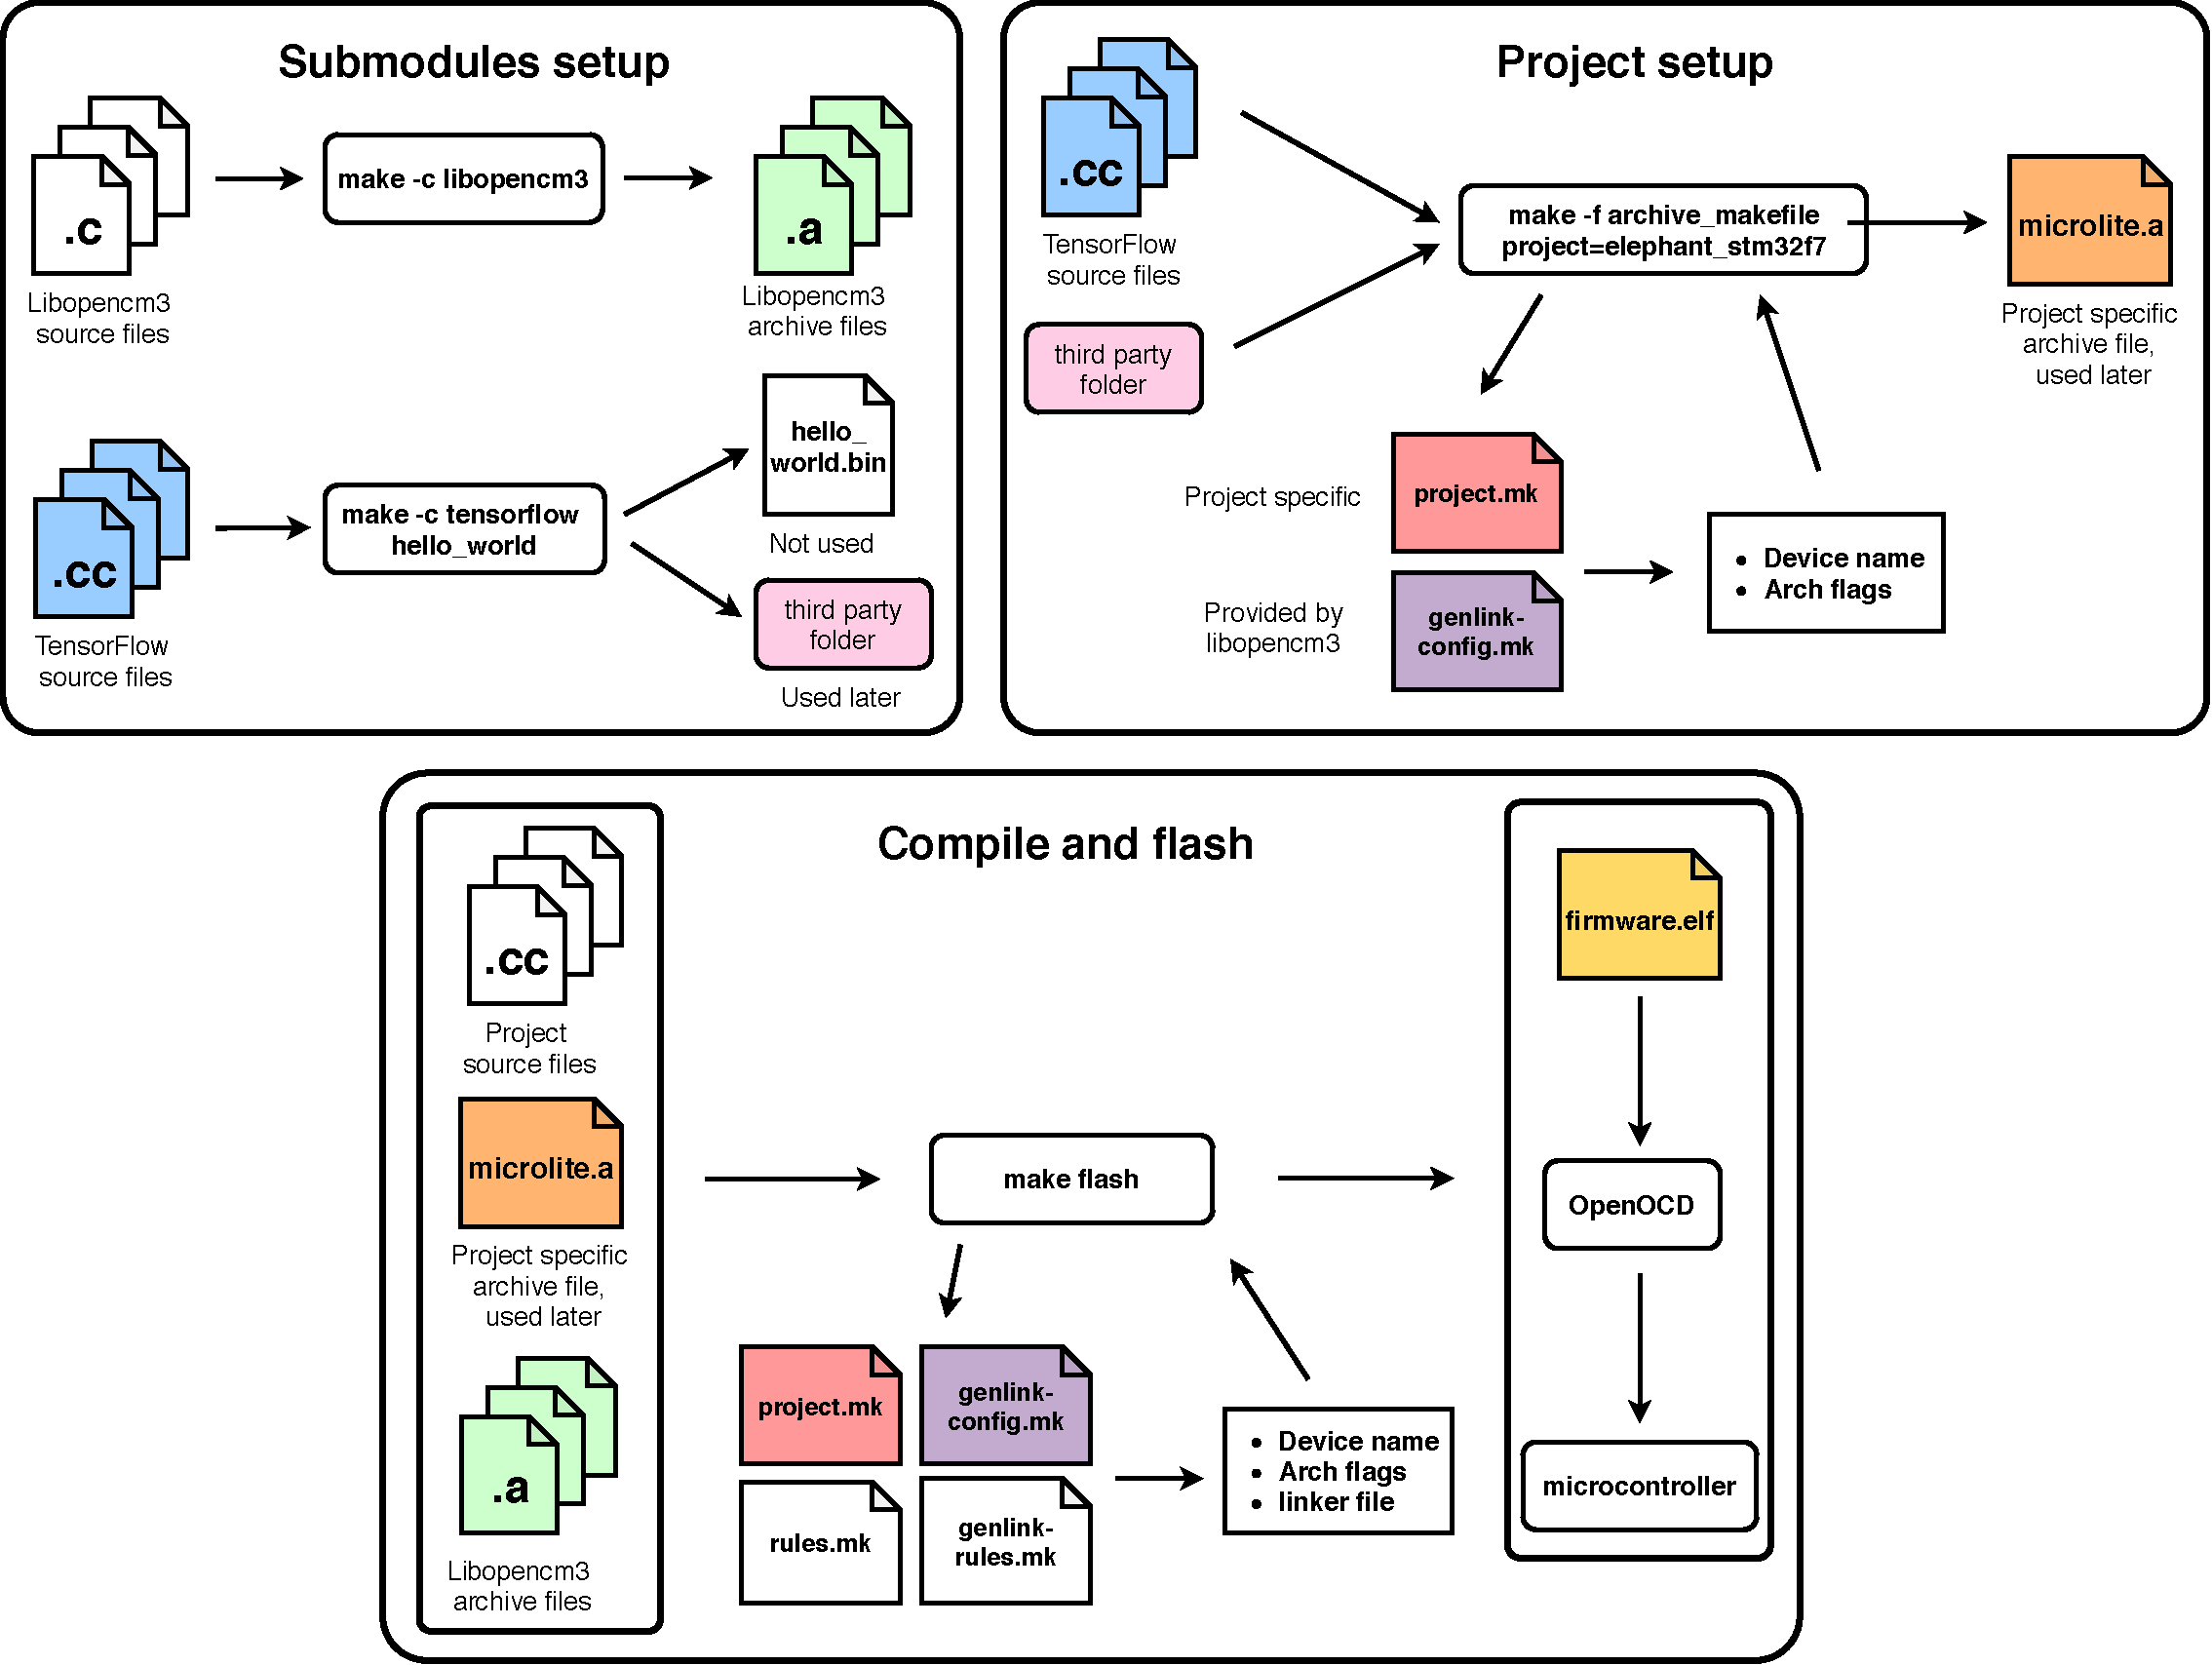
\includegraphics[width=1.0\linewidth]{build_system.pdf} 
        \caption{ Build system of MicroML project.} 
        \label{build_system}
\end{figure}

In \textit{submodules setup} stage we first compile both of the submodules, this step requires two makefiles that are already provided by each submodule.
Compiling libopencm3 creates a group of archive files (static libraries), which contain all platform specific code.
Compiling a TensorFlow Hello World example does not produce any archive files that we would need, however, it does execute several scripts which download several different third party files.
TFLite Micro library depends on these files, which means that MicroML does as well.
\textit{Submodules setup} stage only has to be executed once.

Whenever we start with a new project that will use ML algorithms, we need to go through \textit{project setup} stage.
From main directory, we call \verb|make| command with \verb|archive_makefile| and define \verb|PROJECT| variable with the name of our project.
\verb|Archive_makefile| looks into \verb|project.mk| and extracts \verb|DEVICE| variable.
Libopencm3's \verb|genlink-config.py| script then determines which microcontroller specific compilation flags\footnotemark are needed. 
All needed TensorFlow source files and third party files are then compiled and a project specific \verb|microlite.a| archive file is created in our project's folder.
\footnotetext{ For example, to compile firmware for STM32F767ZI we need flags \verb|-mcpu=cortex-m7|, \verb|-mthumb|, \verb|-mfloat-abi=hard| and \verb|-mfpu=fpv5-sp-d16|.They tell GCC compiler that we are compiling for a cortex-m7 processor, that we want to use thumb instruction set and that we want to use hardware floating-point unit with single precision.}

\textit{Compile and flash} stage is then continuously executed during the development process.
By calling \verb|make flash| directly in our project folder we compile all project files, \verb|microlite.a| and libopencm3 archive files that were created early.
Libopencm3 helper scripts (\verb|genlink-config.mk| and \verb|genlink-rules.mk|) provide us with the microcontroller specific flags and a linker script.
After compilation a \verb|firmvare.elf| is created, Make then automatically calls OpenOCD, which flashes a microcontroller.

As flashing a big binary to a microcontroller takes a long time, we also created a similar setup for testing inference directly on the host machine.
That way we could test ML specific routines fast and quickly remove any mistakes found on the way.


\subsection{ Running inference on a microcontroller}

TFLite Micro API is fairly simple to use and general enough that it can be copied from project to project without many modifications.
Figure \ref{inference_code} shows a simplified inference code example, copied from our project.
\lstset{style=mystyle}
\begin{figure}[ht] 
    \begin{lstlisting}[language=C++]
// An area of memory to use for input, output, 
// and intermediate arrays.
const int kTensorArenaSize = 200 * 1024;
static uint8_t tensor_arena[kTensorArenaSize];

int main() 
{
    // Debug print setup
    tflite::MicroErrorReporter micro_error_reporter;
    tflite::ErrorReporter *error_reporter = &micro_error_reporter;

    // Map the model into a usable data structure
    const tflite::Model* model = tflite::GetModel(full_quant_tflite);

    // Pull in needed operations
    static tflite::MicroMutableOpResolver<8> micro_op_resolver;
    micro_op_resolver.AddConv2D();
    micro_op_resolver.AddMaxPool2D();
    micro_op_resolver.AddReshape();
    micro_op_resolver.AddFullyConnected();
    micro_op_resolver.AddSoftmax();
    micro_op_resolver.AddDequantize();
    micro_op_resolver.AddMul();
    micro_op_resolver.AddAdd();

    // Build an interpreter to run the model with.
    static tflite::MicroInterpreter interpreter(model, 
                                                micro_op_resolver, 
                                                tensor_arena,
                                                kTensorArenaSize, 
                                                error_reporter);
    // Allocate memory from the tensor_arena
    interpreter->AllocateTensors();

    // Get information about the memory area 
    // to use for the model's input.
    TfLiteTensor* input  = interpreter->input(0);
    TfLiteTensor* output = interpreter->output(0);

    // Load data from image array
    for (int i = 0; i < input->bytes; ++i) {
        input->data.int8[i] = image_array[i];
    }

    // Run the model on this input and time it
    uint32_t start = dwt_read_cycle_counter();
    interpreter->Invoke();
    uint32_t end   = dwt_read_cycle_counter();
    
    // Print probabilites and time elapsed
    print_result(error_reporter, output, dwt_to_ms(end-start));
}
    \end{lstlisting}
    \caption{ Example of TensorFlow Lite inference code in C++.}
    \label{inference_code}
\end{figure}
\clearpage
As a first step, we need to define the size of \verb|tensor_arena| array, which holds memory of input, output, and intermediate arrays.
Exact size of \verb|tensor_arena| is determined by trail and error: we set it to some big value and then decrease it in steps, until the code does not work any more.

In lines 9 and 10 we create an instance of \verb|ErrorReporter| object.
This object serves as a thin wrapper around platform specific \verb|printf| implementation.
If some part of TensorFlow code crashes, \verb|ErrorReporter| notifies us what went wrong.

In the line 13 we pull in our ML model in hex dump format that we created with xxd.
\verb|Full_quant_model| is defined in a different file, not seen in this example.

In lines 16 to 24 we create an operation resolver.
One way to do it is to specify each required operation specifically (which is done in the example) or simply pull in all operations.
Latter approach is not recommended, as it results in large binary size.
To find out exactly which operations were required we used online tool Netron\cite{netron}, which showed us a deconstructed view of a trained model.

In lines 27 and 33 we create an \verb|MicroIinterpreter| instance and allocate memory to it that we specified with \verb|tensor_arena| earlier.
Lines 37 and 38 assign input and output of the interpreter to the new \verb|TfLiteTensor| variables.
This step enables us to do two things.
Firstly, variables \verb|input| and \verb|output| now point to information about data format: We can found out how many dimensions are needed, what is the size of those dimensions and what is expected type of variable (\verb|uint8_t|, \verb|int8_t|, \verb|float|...).
In tests that we were running on the laptop, we tested exactly for these values to confirm that the model works as expected.
Secondly, we now have a way to directly feed data into input, this is done in for loop on line 41.
One of \verb|TfLiteTensor| members is a union variable \verb|data| which contains variables of all possible types.
This type of structure enables us to load input with any kind of data, in our case \verb|int8|.

In line 47 we finally invoke interpreter and run inference on input data.
The whole expression is surrounded by the timing functions, which are used to keep track of time spent computing inference.

We finally call \verb|print_results|, written by us, where we pass \verb|error_reporter| for printing, \verb|output| for extracting computed probabilities and elapsed time.

After the initial setup, we can load data, call invoke, and print results as many times we want.


\section{ Server-side components and software}

In this section, we describe possible server-side construction of various frameworks which enable us to receive LoRaWAN messages, parse them, store them in a database and visualise them.
We did not implement this specific setup as it was not required for testing purposes, however, at IRNAS we use this setup constantly for our IoT products and implementation of a such system would be trivial.

The system that we use consists of different tools, each one with a distinct task.
These tools are The Things Network (TTN), Node-RED, InfluxDB and Grafana.
The flow of information and tasks for each tool is presented in Figure \ref{server_side}.

\begin{figure}[ht]
    \centering
    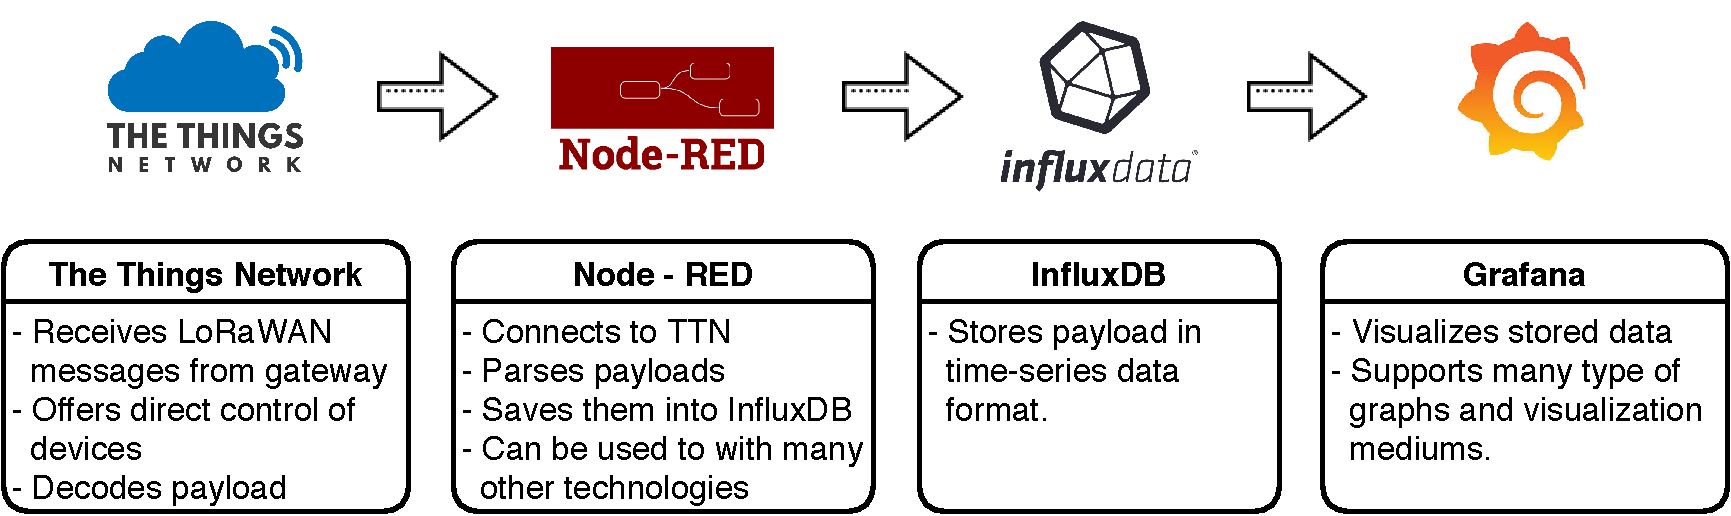
\includegraphics[width=1.0\linewidth]{server_side.pdf} 
    \caption[Server side flow of information.]{Server side flow of information. Icons source:\cite{icons}}
    \label{server_side}
\end{figure}

TTN is responsible for routing packets that are captured by a gateway to the application server.
Since it is open-source and free, anyone can register their gateway device into the network and thus helping to extend it.
TNN is web-based, so we can see payload messages directly in the browser.
Since data is usually encoded in binary format, we can provide a decoder-script written in JavaScript and TTN will automatically pass each message, thus decoding it.

Node-RED functions as a glue logic that parses packets and shapes them into a format that is required by InfluxDB.
Node-RED provides a browser-based flow editor, where actual programming can be done graphically.
Logic is programmed by choosing different blocks called \textit{nodes} and connecting them.
This is convenient, as Node-RED provides different nodes for communicating with different technologies, such as MQTT, HTTP requests, emails, Twitter accounts and others.
In our use case, we needed to use nodes seen in Figure \ref{nodered_flow}.
Node \textit{Elephant Gateway} is connected to a specific application on TTN, which is used for the collection of packets from our devices in the field.
Any packet that will appear in that TTN application will also appear in Node-RED.
Node \textit{Parse packet} extracts the information contained in each packet and stores it in a specific format, which is finally sent to the node \textit{Elephant Database}.

\begin{figure}[ht]
    \centering
    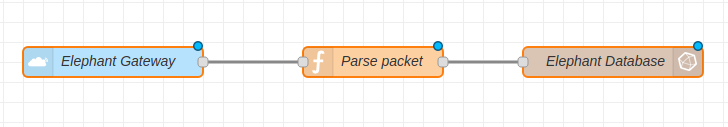
\includegraphics[width=1.0\linewidth]{nodered_flow.png} 
    \caption{ Node-RED flow}
    \label{nodered_flow}
\end{figure}

\textit{Elephant Database} is connected to InfluxDB, which acts as a time-series database.
Any packet that is saved in it is automatically timestamped.

Data is then visualized in Grafana. 
Grafana is an open-source analytics and monitoring solution.
Users define which database is set as a source and Grafana provides graphical controls which are at some point converted into SQL-like language, understandable to InfluxDB.
Grafana provides different types of visualizations, such as graphs, gauges, heat maps, alert lists and others.
In our use case, we could display information about various devices in the field, such as battery voltage, number of wakeup triggers, results of each inference and others.

Example of Grafana graph can be seen in Figure \ref{grafana}.
\clearpage
\begin{figure}[ht]
    \centering
    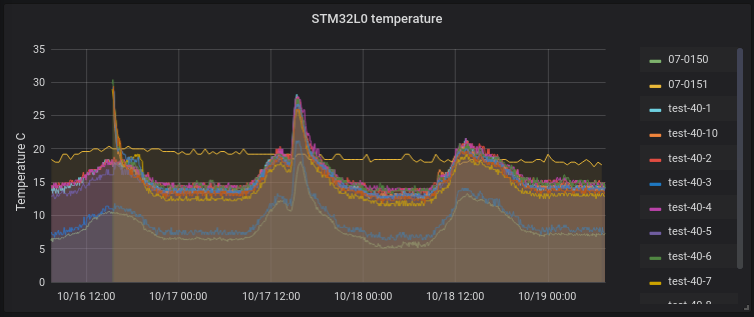
\includegraphics[width=1.0\linewidth]{grafana.png} 
    \caption{ Example of Grafana graph.}
    \label{grafana}
\end{figure}

One important quality of Node-RED, InfluxDB and Grafana is that they can run directly on an embedded Linux system, such as Raspberry Pi or BeagleBone, which greatly lowers the cost of hardware that is needed.
